
\documentclass[titlepage, a4paper]{article}
\usepackage[swedish]{babel}
\usepackage[utf8]{inputenc}
\usepackage{color}

% Sidformat
\usepackage{a4wide}

% Fixa Appendix-titlar
\usepackage[titletoc,title]{appendix}

% Bättre bildtexter
\usepackage[margin=10pt,font=small,labelfont=bf,labelsep=endash]{caption}

% Enkelt kommando som låter mig attgöra-markera text
\newcommand{\todo}[1] {\textbf{\textcolor{red}{#1}}}

%% Headers och Footers
\usepackage{fancyhdr}
\pagestyle{fancy}
\lhead{}
\rhead{\today}
\lfoot{\LIPSkursnamn \\ \LIPSdokumenttyp}
\cfoot{\thepage}
\rfoot{\LIPSprojektgrupp \\ \LIPSprojektnamn}

%% Titelsida
\newcommand{\LIPSTitelsida}{%
{\ }\vspace{45mm}
\begin{center}
  \textbf{\Huge \LIPSdokument}
\end{center}
\begin{center}
  {\Large Redaktör: \LIPSredaktor}
\end{center}
\begin{center}
  {\Large \textbf{Version \LIPSversion}}
\end{center}
\vfill
\begin{center}
  {\large Status}\\[1.5ex]
  \begin{tabular}{|*{3}{p{40mm}|}}
    \hline
    Granskad & \LIPSgranskare & \LIPSgranskatdatum \\
    \hline
    Godkänd & \LIPSgodkannare & \LIPSgodkantdatum \\
    \hline
  \end{tabular}
\end{center}
\newpage
}


% Projektidentitet
\newenvironment{LIPSprojektidentitet}{%
{\ }\vspace{45mm}
\begin{center}
  {\Large PROJEKTIDENTITET}\\[0.5ex]
  {\small
  \LIPSartaltermin, \LIPSprojektgrupp\\
  Linköpings Tekniska Högskola, MAI
  }
\end{center}
\begin{center}
  {\normalsize Gruppdeltagare}\\
  \begin{tabular}{|l|l|p{25mm}|l|}
    \hline
    \textbf{Namn} & \textbf{Ansvar} & \textbf{Telefon} & \textbf{E-post} \\
    \hline
}%
{%
    \hline
  \end{tabular}
\end{center}
\begin{center}
  {\small
    \textbf{E-postlista för hela gruppen}: \LIPSgruppadress\\
    \textbf{Hemsida}: \LIPSgrupphemsida\\[1ex]
    \textbf{Kund}: \LIPSkund\\
    \textbf{Kontaktperson hos kund}: \LIPSkundkontakt\\
    \textbf{Kursansvarig}: \LIPSkursansvarig\\
    \textbf{Handledare}: \LIPShandledare\\
  }
\end{center}
\newpage
}
\newcommand{\LIPSgruppmedlem}[4]{\hline {#1} & {#2} & {#3} & {#4} \\}

%% Dokumenthistorik
\newenvironment{LIPSdokumenthistorik}{%
\begin{center}
  Dokumenthistorik\\[1ex]
  %\begin{small}
    \begin{tabular}{|l|l|p{60mm}|l|l|}
      \hline
      \textbf{Version} & \textbf{Datum} & \textbf{Utförda förändringar} & \textbf{Utförda av} & \textbf{Granskad} \\
      }%
    {%
			\hline
    \end{tabular}
  %\end{small}
\end{center}
}

\newcommand{\LIPSversionsinfo}[5]{\hline {#1} & {#2} & {#3} & {#4} & {#5} \\}

% Kravlistor
\newenvironment{LIPSkravlista}{
	\center
		\tabularx{\textwidth}{| p{1.2cm} | p{1.9cm} | X | c |}
			\hline
			\textbf{Krav} & \textbf{Förändring} & \textbf{Beskrivning} & \textbf{Prioritet} \\\hline
}
{
		\endtabularx
	\endcenter
}

\newcounter{LIPSkravnummer}
\addtocounter{LIPSkravnummer}{1}
\newcommand{\LIPSkrav}[4][Krav \arabic{LIPSkravnummer}]{{#1} & {#2} & {#3} & {#4} \stepcounter{LIPSkravnummer}\\\hline}	% Importera generella layout-strukturer

% Information nödvändig för generella layout-strukturer
\newcommand{\LIPSredaktor}{Hannes Snögren}
\newcommand{\LIPSversion}{0.1}
\newcommand{\LIPSdokument}{Designspecifikation}
\newcommand{\LIPSdokumenttyp}{Designspecifikation}
\newcommand{\LIPSgranskatdatum}{}
\newcommand{\LIPSgranskare}{}
\newcommand{\LIPSgodkannare}{}
\newcommand{\LIPSgodkantdatum}{}
\newcommand{\LIPSkursnamn}{TSEA29}
\newcommand{\LIPSprojektnamn}{Lagerrobot}
\newcommand{\LIPSprojektgrupp}{Grupp 2}
%\newcommand{\LIPSgruppadress}{}
\newcommand{\LIPSartaltermin}{HT1, 2014}	
\newcommand{\LIPSgrupphemsida}{http://github.com/ultralaserdeluxe/gloria}
\newcommand{\LIPSkund}{Tomas Svensson}
\newcommand{\LIPSkundkontakt}{Tomas Svensson}
\newcommand{\LIPSkursansvarig}{Tomas Svensson}
\newcommand{\LIPShandledare}{Peter Johansson}

% Dokument-specifika paket
\usepackage{tabularx}
\usepackage{subcaption}
\usepackage{tikz}
\usepackage{mathtools}
\usetikzlibrary{shapes, arrows}

\pagenumbering{roman}

\begin{document}

\LIPSTitelsida

\begin{LIPSprojektidentitet}
\LIPSgruppmedlem{Pål Kastman}{Projektledare}{0703896295}{palka285@student.liu.se}
\LIPSgruppmedlem{Hannes Snögren}{Dokumentansvarig}{0706265064}{hansn314@student.liu.se}
\LIPSgruppmedlem{Alexander Yngve}{Hårdvaruansvarig}{0762749762}{aleyn573@student.liu.se}
\LIPSgruppmedlem{Martin Söderén}{Mjukvaruansvarig}{0708163241}{marso329@student.liu.se}
\LIPSgruppmedlem{Daniel Wassing}{Leveransansvarig}{0767741110}{danwa223@student.liu.se}
\LIPSgruppmedlem{Dennis Ljung}{Testansvarig}{0708568148}{denlj069@student.liu.se}
\end{LIPSprojektidentitet}

\newpage
\tableofcontents	%Innehållsförteckning	
%\listoffigures
%\listoftables

\newpage

\begin{LIPSdokumenthistorik}
\LIPSversionsinfo{0.1}{}{}{}{}
\end{LIPSdokumenthistorik}

\newpage
\pagenumbering{arabic}	%Påbörja sidnumrering

% Inledning, översikt osv
\section{Inledning}
Systemet kommer bestå av en robot som i sig består av tre undermoduler. Utöver detta tillkommer mjukvara på roboten och PC som används för manuell styrning och övervakning. Detta är en systemskiss som ska ge en grov översikt hur systemet ska implementeras. Detta ska sedan vara underlag för designspecifikationen. 
\newline
\newline
Varje enskild modul kommer att ha en egen processor och dessa kommer sedan kommunicera med varandra. Systemet kommer kommunicera med en PC över blåtand. När systemet är klart för leverans ska det kunna följa en bana som visas nedan (figur \ref{systemskiss:banoversikt}) och plocka upp och sätta ned paket på de utsatta stationerna B och C. Den ska även kunna detektera avbrott (A) samt slutstation (D). 

\begin{figure}[h]
\center
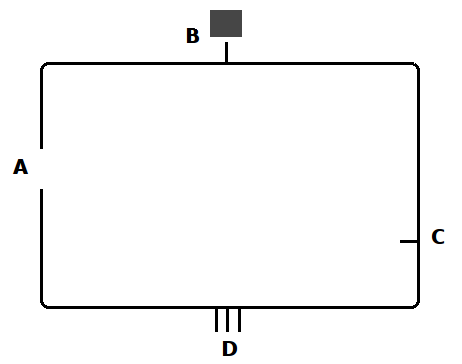
\includegraphics[scale=0.4]{figur}
\caption{Banöversikt.} \label{systemskiss:banoversikt}
\end{figure}

\begin{figure}[h]
\center
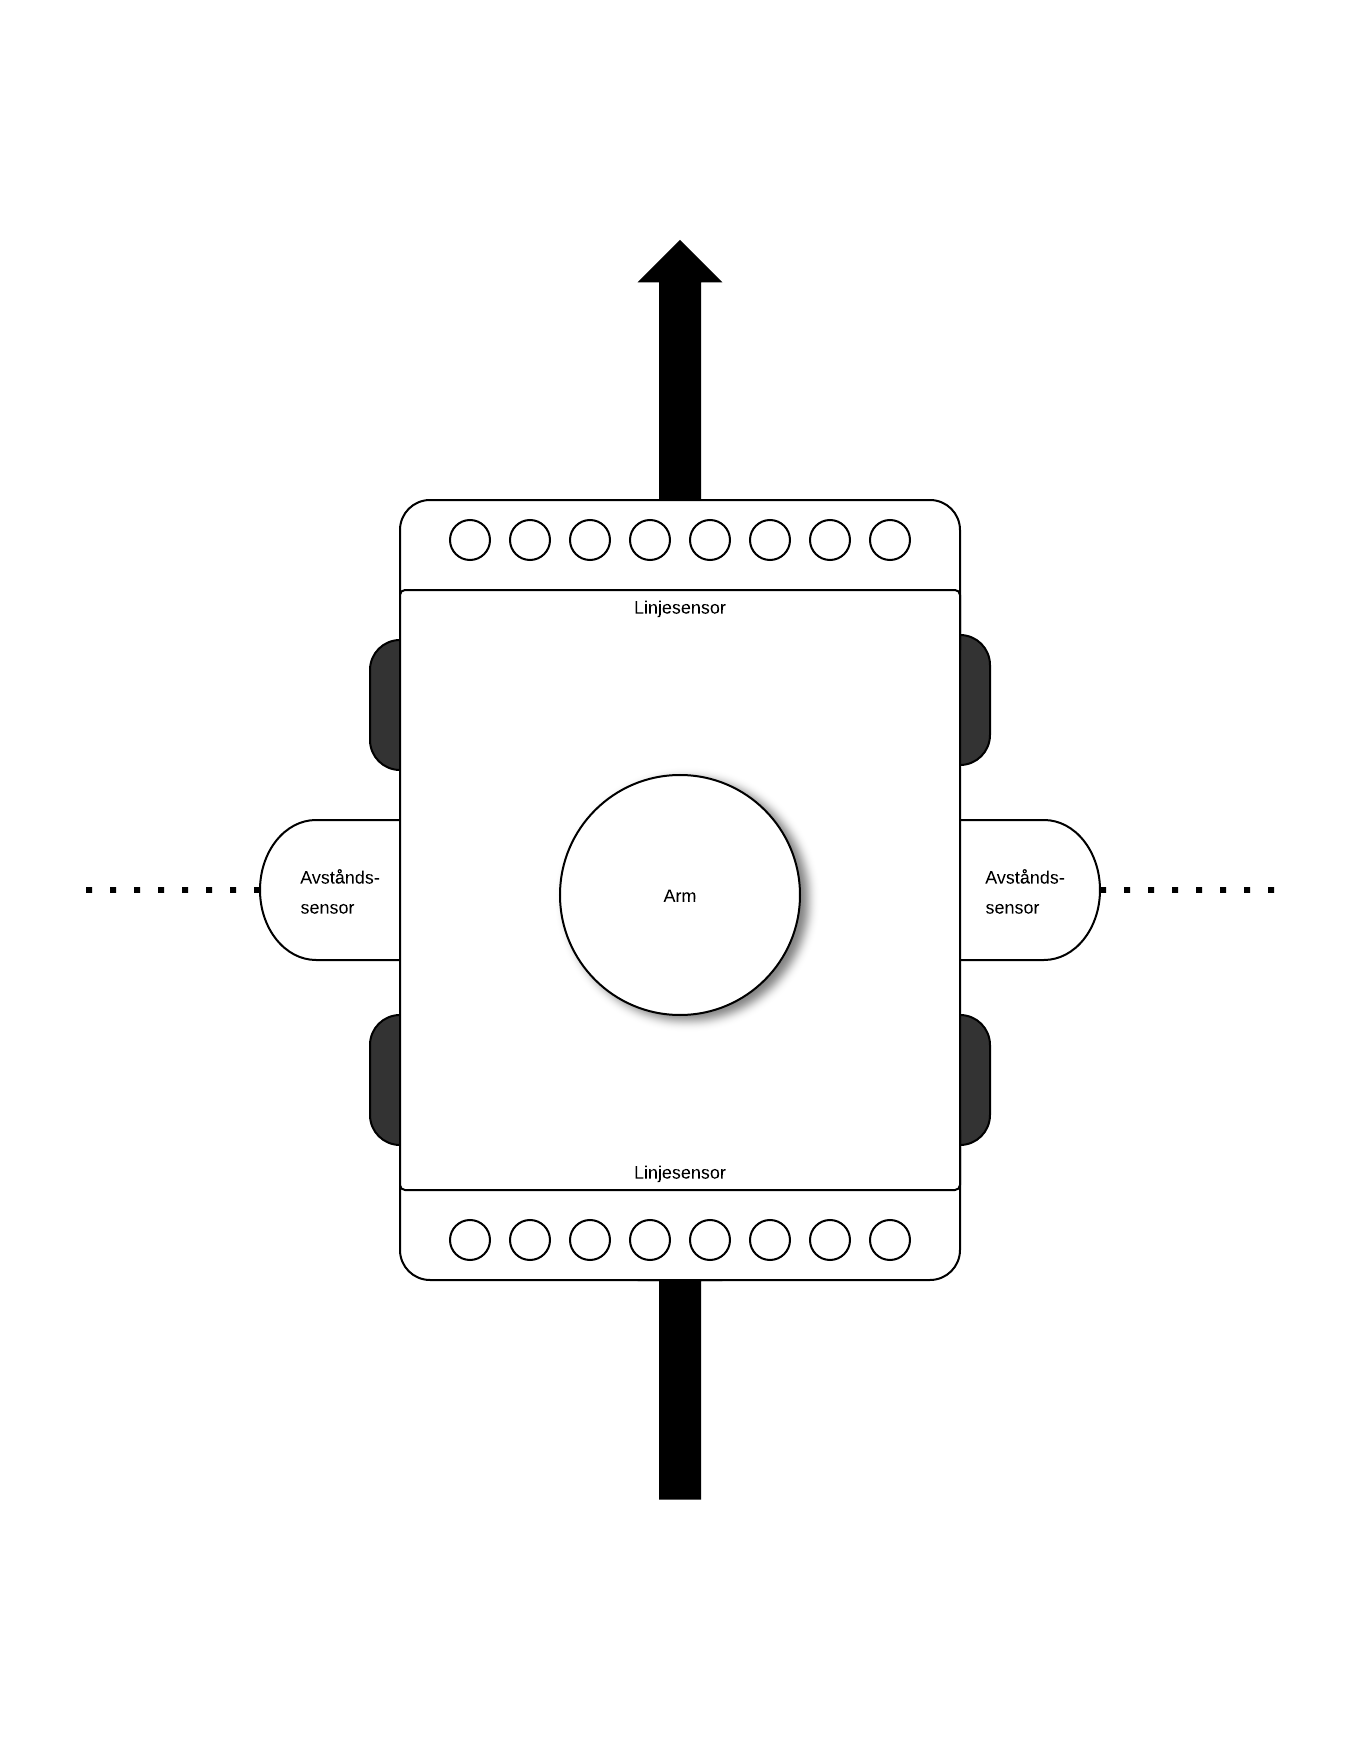
\includegraphics[scale=0.15]{robot}
\caption{Robot sedd ovanifrån.} \label{designspec:robot}
\end{figure}
\todo{Rita om figur \ref{designspec:robot}}

%\centerline{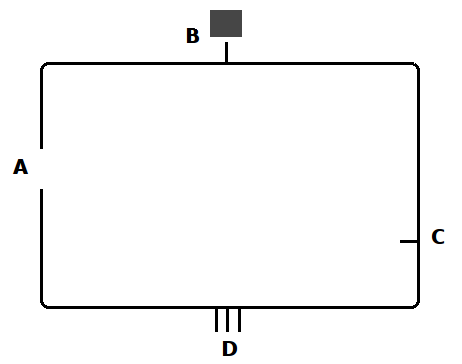
\includegraphics[scale=0.4]{figur}}
%\centerline{Banöversikt}
%\centerline{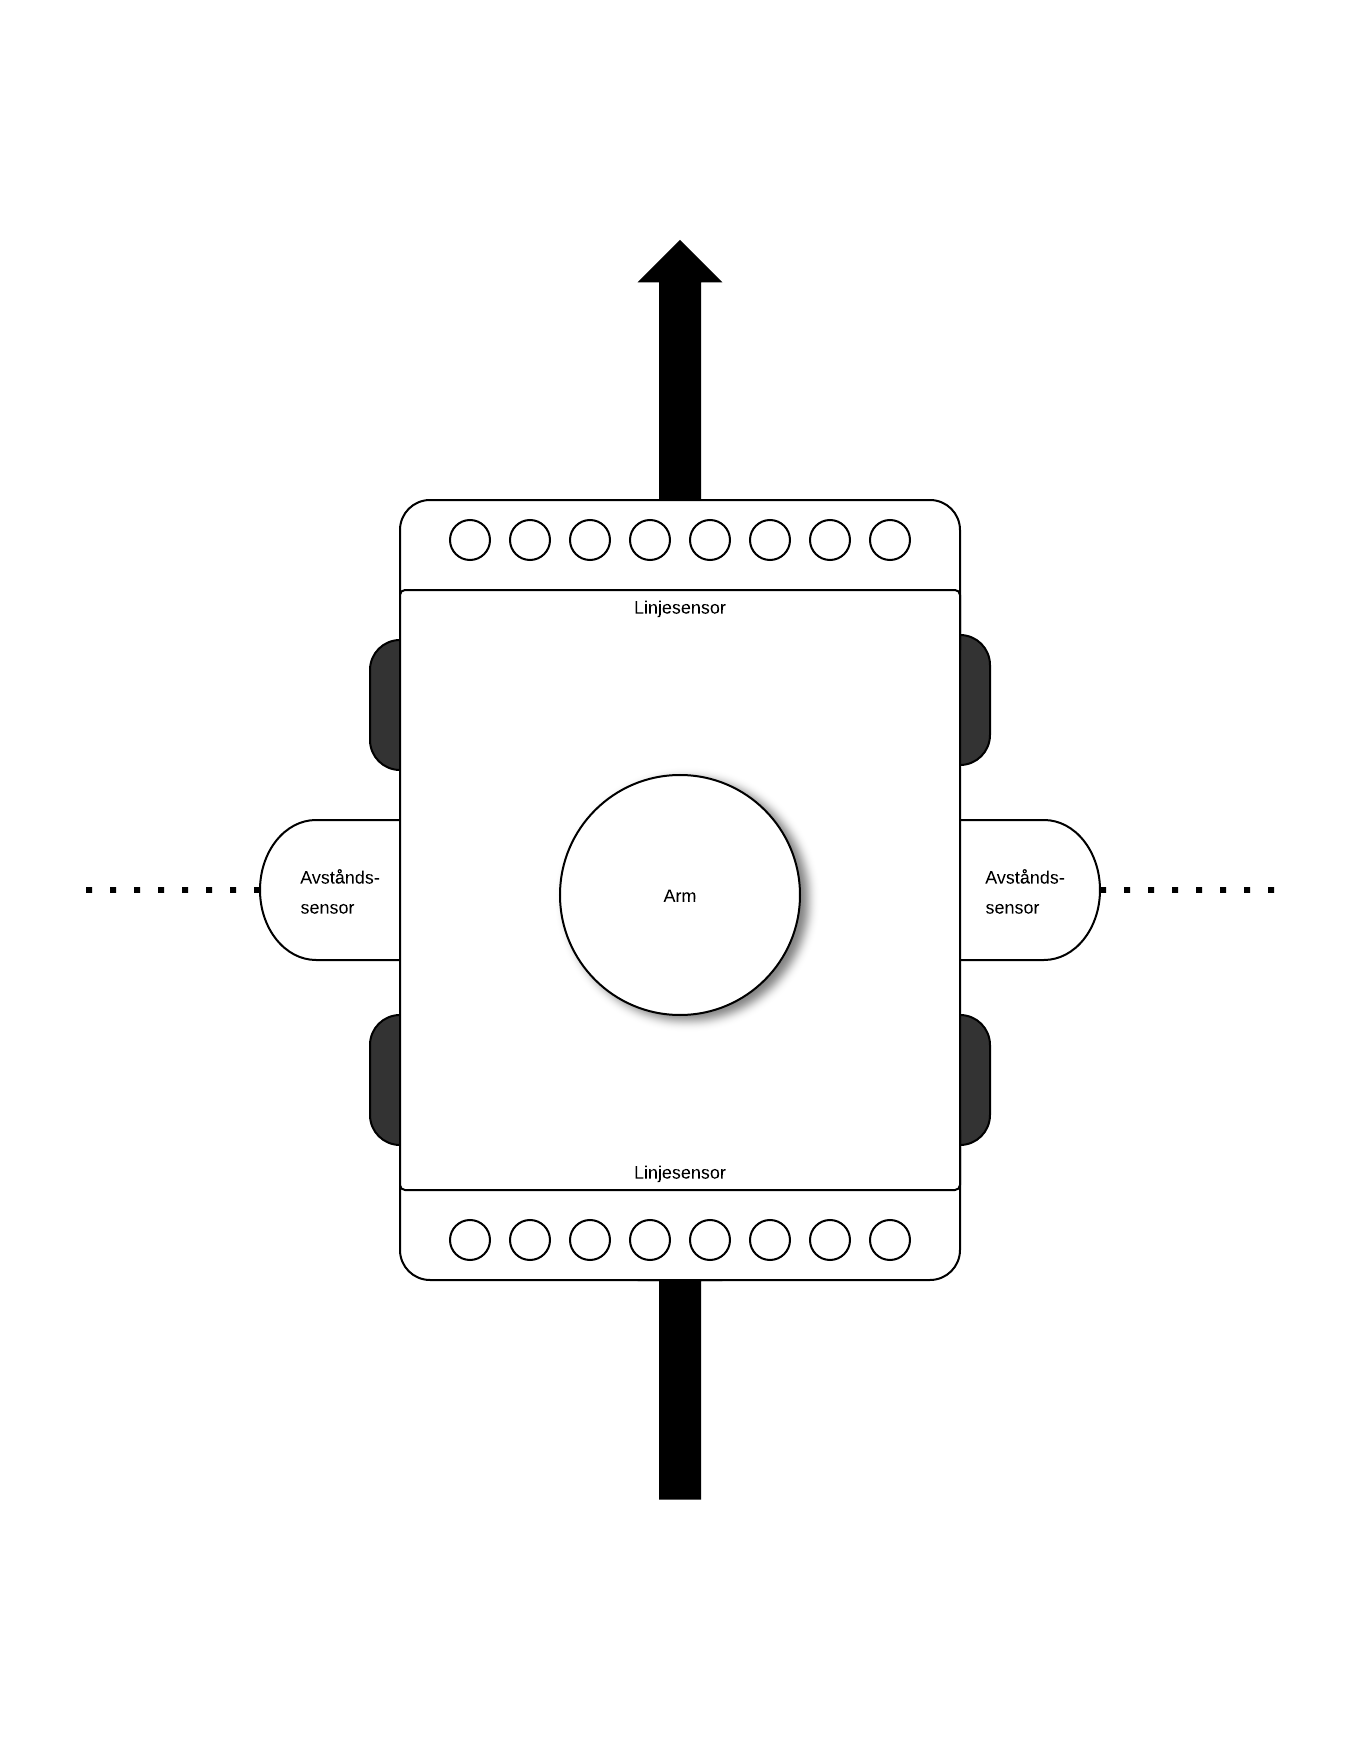
\includegraphics[scale=0.19]{robot}}
%\centerline{Robot sedd ovanifrån}	

\section{Översikt av system}
Plattformen består av sammanlagt fyra enheter. En PC-enhet, en huvudenhet, en sensorenhet och en styrenhet. \\
PC-enheten är framförallt ett användargränssnitt som gör det enkelt för användaren att styra roboten och robotarmen men fungerar även som ett debugverktyg där användaren kan se robotens status och debuginformation. Huvudenheten står för huvuddelen av alla beräkningar roboten behöver göra så som regleringsalgoritm för linjeföljaren och koordinatkonvertering för armen. Sensorenheten innehåller den funktionalitet som krävs för att driva alla systemets sensorer och styrenheten innehåller den funktionalitet som krävs för att köra motorer och servon.

\subsection{Kommunikationskanaler}
I det fall att roboten arbetar i manuellt läge, skickar PC-enheten kommandon till huvudenheten över Blåtand. I annat fall arbetar roboten autonomt och PC-enheten skickar endast förfrågningar angående robotens status. Huvudenheten skickar kommandon till sensorenheten och styrenheten över en SPI-buss.

\subsection{Uppgraderbarhet}
Kommunikation mellan huvudmodulen och PC-enheten kommer att ske över Blåtand och kommer att användas för att sätta upp ett PAN. Över denna sätts en TCP/IP anslutning upp och data skickas över en Python-socket vilket leder till att bluetooth kan bytas ut mot till exempel WIFI, en ethernetkabel eller annan överföringskanal som tillåter TCP/IP. \\
Kommunikationen mellan huvudmodulen och styrenheten samt sensormodulen sker över en SPI-buss med ett väldefinierat protokoll. Om det önskas kan sensormodulen och styrmodulen bytas ut mot andra moduler så länge de använder samma protokoll. Styrenheten kommunicerar med servona över UART och använder ett protokoll speciellt för Trossenrobotics Reactor vilket leder till att armen inte kan bytas ut mot någon annan.

\begin{figure}[h!]
\center
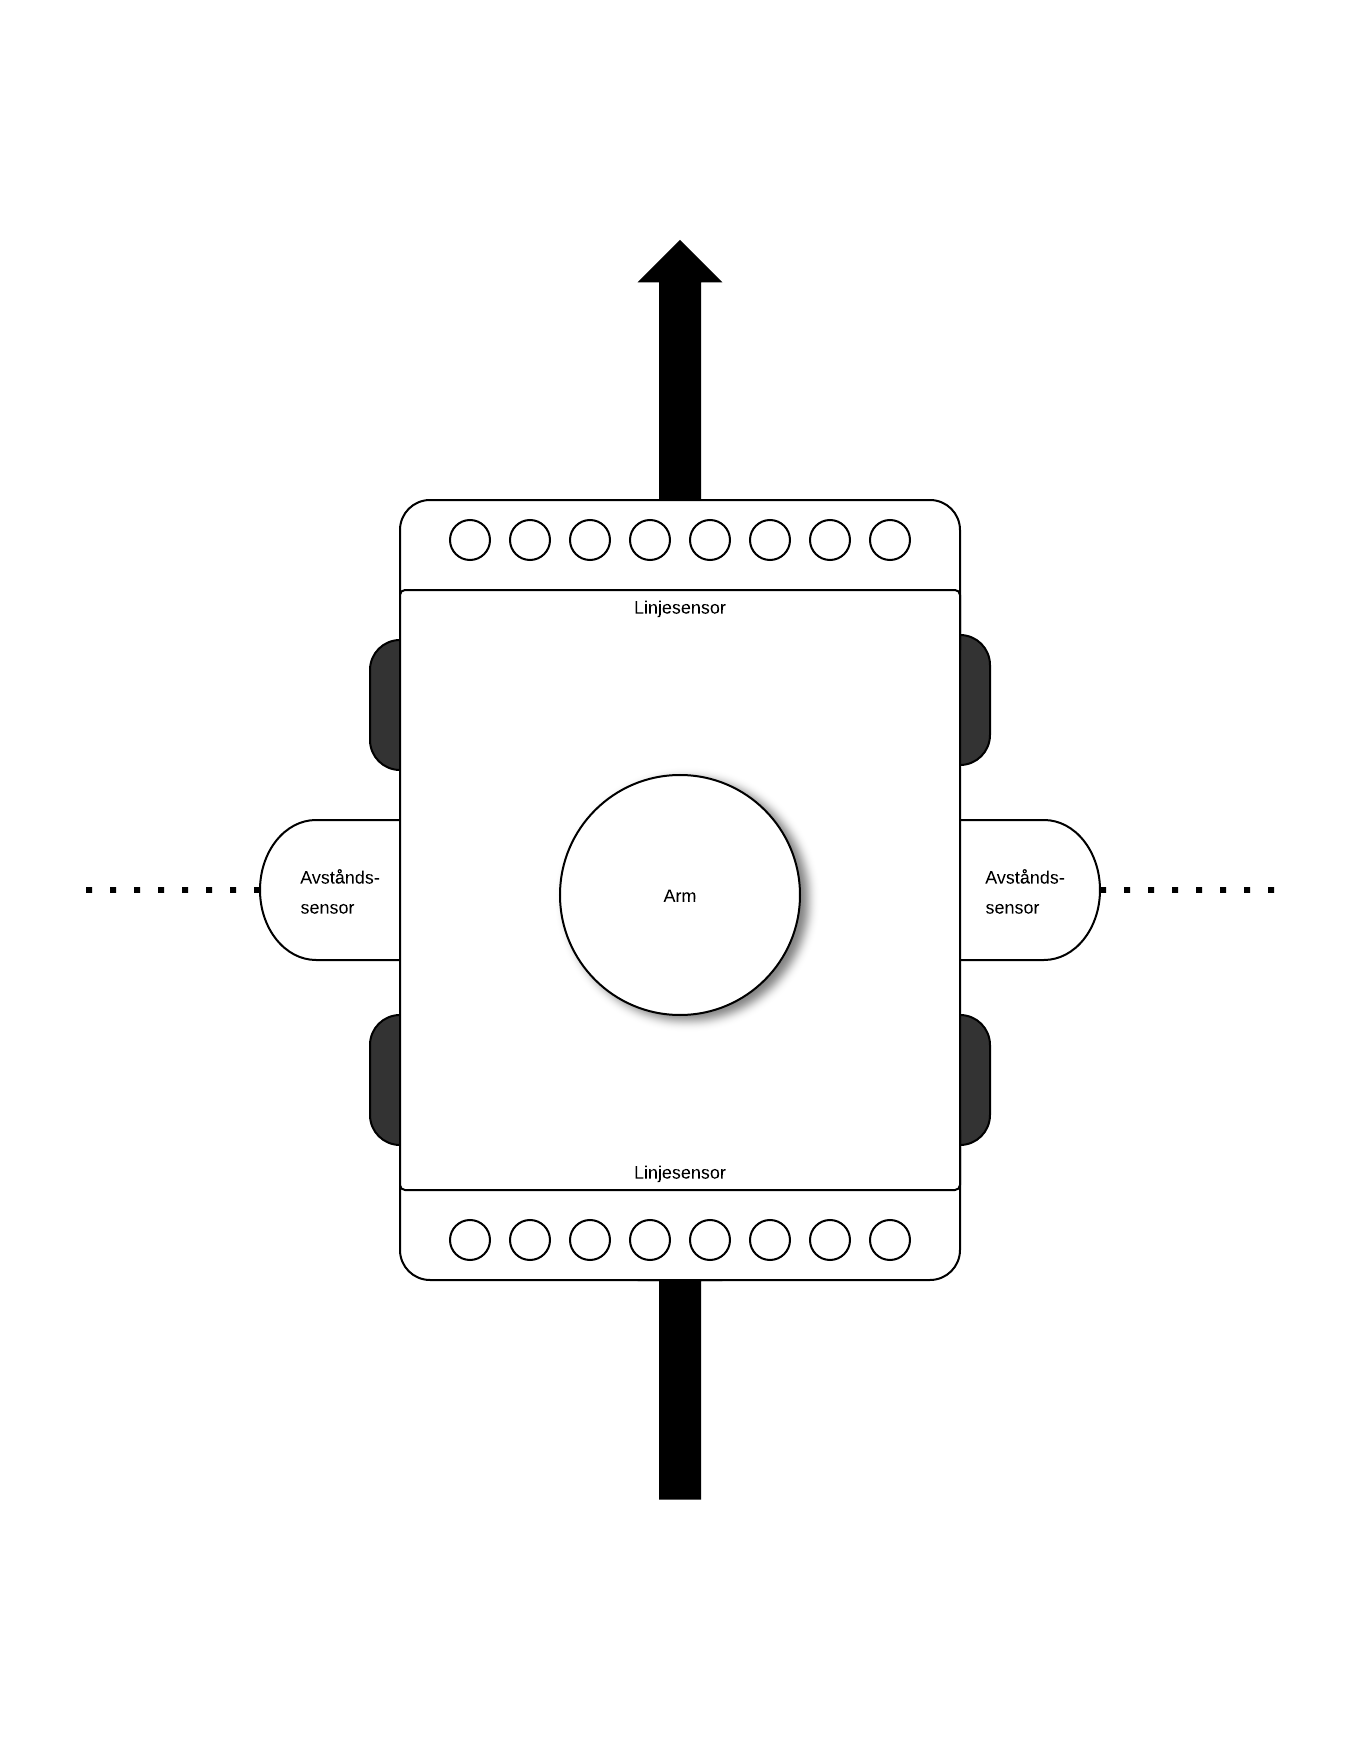
\includegraphics[scale=0.32]{robot}
\caption{Översikt över roboten} \label{designspec:robot}
\end{figure}

\section{Protokoll för kommunikation}

\subsection{Kommunikation mellan PC och huvudmodul}\label{designspec:protokoll}

Kommunikation mellan PC-enhet och huvudenhet sker via Blåtand. En instruktion ges som en sträng på formen $command1=arg1,...,argN;command2=arg1,...,argN$ med ett godtyckligt antal instruktioner där antalet argument per instruktion specificeras i avsnitt \ref{designspec:protokoll-pc-huvud-kommandon}.

\subsubsection{Instruktioner} \label{designspec:protokoll-pc-huvud-kommandon}

\begin{table}[h]
	\centering
		\begin{tabularx}{\textwidth}{| l | l | X |}
			\hline
			\textbf{Instruktion} & \textbf{Argument} & \textbf{Beskrivning} \\
			\hline
			{motor} & {L,R} & {L och R anger hastigheten på det vänstra, respektive högra hjulparet} \\
			\hline
			{arm} & {X,Y,Z,P,G} & {X,Y,Z är koordinaten i rummet dit armens hand skall röra sig. Armens fundament är origo, P anger handens vinkel i förhållande till Z-axeln och G anger avståndet mellan handens fingrar.} \\
			\hline
			{calibrate} & {} & {Begär kalibrering av robotens sensorer} \\
			\hline
			{status} & {} & {Begär statusrapport från robot} \\
			\hline
			{automotor} & {M} & {Ange om robotens motorer skall styras från PC-enheten (0) eller huvudenheten (1)} \\
			\hline
			{autoarm} & {M} & {Ange om robotarmen skall styras från PC-enheten (0) eller huvudenheten (1)} \\
			\hline
			{start} & {} & {Initiera körning} \\
			\hline
		\end{tabularx}
	\caption{Instruktioner från PC-enhet till huvudenhet} \label{protokoll:pc-huvud}
\end{table}
%\todo{Högre/lägre värden på t.ex X eller P gör vad, precis? X och Y =-+38cm,0<=Z<=46 bestäm upplösning}\\
%\todo{Illustrera koordinatsystem m. bild}
L och R:s begränsningar där 100 representerar maximal hastighet framåt och -100 representerar maximal hastighet bakåt
$$-100\leq L \leq 100$$
$$-100\leq R \leq 100$$
Begränsningar på X,Y,Z motsvarar hur långt roboten kan sträcka sig i varje led
$$-3800\leq X \leq 3800$$
$$-3800\leq Y \leq 3800$$
$$0\leq Z \leq 4600$$
Begränsningarna på G motsvarar servots input för position
$$0\leq G \leq 1024$$
Begränsningarna på P motsvarar vilken vinkel robotens hand kan ha mot XY planet.
$$-90\leq P \leq 90$$

\todo{Bygg om}

\subsection{Kommunikation mellan huvudmodul och sensormodul}
Kommunikation mellan huvudmodul och sensormodul sker via en SPI-buss. Instruktioner från huvudmodulen ges i form av en byte. De fyra första bitarna anger vilken instruktion som skall utföras. De sista fyra anger vilken sensor instruktionen gäller. Tabell \ref{protokoll:huvud-sensor} och \ref{protokoll:huvud-sensor-adress} under avsnitt \ref{designspec:protokoll-huvud-sensor-instr} specificerar de instruktioner som finns respektive vilken adress som avser vilken sensor. \\
Sensorenheten svarar med endast data. En byte per fototransistor i linjesensorn. En byte för vardera avståndssensor. I fallet med instruktionen \textit{läs data från alla sensorer} skickas sensorernas data seriellt i följande ordning: 1. Linjesensor, 2: Avståndssensor Höger, 3: Avståndssensor Vänster.

\subsubsection{Instruktioner} \label{designspec:protokoll-huvud-sensor-instr}

\begin{table}[h]
	\centering
		\begin{tabularx}{\textwidth}{| l | l | X |}
			\hline
			\textbf{Instruktion} & \textbf{Argument} & \textbf{Beskrivning} \\
			\hline
			{0000} & {A} & {Returnera sensordata för A} \\
			\hline
			{0001} & {A} & {Kalibrera sensor A} \\
			\hline
		\end{tabularx}
	\caption{Instruktioner från huvudenhet till sensorenhet} \label{protokoll:huvud-sensor}
\end{table}

\begin{table}[h]
	\centering
		\begin{tabularx}{\textwidth}{| l | X |}
			\hline
			\textbf{Adress} & \textbf{Beskrivning} \\
			\hline
			{0000} & {Linjesensor Fram} \\
			\hline
			{0010} & {Avståndssensor Höger} \\
			\hline
			{0011} & {Avståndssensor Vänster} \\
			\hline
			{1111} & {Adressera samtliga sensorer} \\
			\hline
		\end{tabularx}
	\caption{Adresser för instruktioner till sensorenhet} \label{protokoll:huvud-sensor-adress}
\end{table}

\subsection{Kommunikation mellan huvudenhet och styrenhet} \label{protokoll:pc-motor}
Kommunikation mellan huvudmodul och motormodul sker via en SPI-buss. Det finns en busy-flagga kopplad till huvudmodulen som går låg när armen är i rörelse. \\
En instruktion består av tre bytes. Den första byten innehåller instruktionen och vilket servo eller vilken motor som avses. De första fyra bitarna av denna byte definierar vilket kommando som skall utföras. De nästkommande fyra vilken enhet det skall utföras av. Tabell \ref{protokoll:pc-motor-tabell} och \ref{protokoll:pc-motor-adress-tabell} i avsnitt \ref{designspec:protokoll-pc-motor-instr} specificerar de instruktioner som finns och vilken adress som avser vilken motor eller servo. Efter instruktions-byten följer alltid två databytes. I de fall där endast en databyte är nödvändig används endast den första av databytesen. Oanvända databytes kasseras utan att tolkas av styrenheten.

\subsubsection{Instruktioner} \label{designspec:protokoll-pc-motor-instr}

\begin{table}[h]
	\centering
		\begin{tabularx}{\textwidth}{| l | l | X |}
			\hline
			\textbf{Instruktion} & \textbf{Argument} & \textbf{Beskrivning} \\
			\hline
			{0000} & {} & {Stoppa samtliga servon och motorer} \\
			\hline
			{0001} & {A, D} & {Sätt register A till D} \\
			\hline
			{0010} & {A} & {Utför givna kommandon för A} \\
			\hline
		\end{tabularx}
	\caption{Kommandon från huvudenhet till styrenhet} \label{protokoll:pc-motor-tabell}
\end{table}

\begin{table}[h]
	\centering
		\begin{tabularx}{\textwidth}{| l | X |}
			\hline
			\textbf{Adress} & \textbf{Beskrivning} \\
			\hline
			{0000} & {Höger hjulpar} \\
			\hline
			{0001} & {Vänster hjulpar} \\
			\hline
			{0010} & {Arm axel 1} \\ % Armens bas?
			\hline
			{0100} & {Arm axel 2} \\
			\hline
			{0110} & {Arm axel 3} \\
			\hline
			{1000} & {Arm axel 4} \\
			\hline
			{1011} & {Arm axel 5(gripper)} \\ % Gripklo?
			\hline
			{1100} & {Samtliga motorer} \\
			\hline
			{1101} & {Samtliga servon} \\
			\hline
			{1111} & {Samtliga motorer och servon} \\
			\hline
		\end{tabularx}
	\caption{Adresser för adressering till styrenhet} \label{protokoll:pc-motor-adress-tabell}
\end{table}

\begin{figure}[h]
\centerline{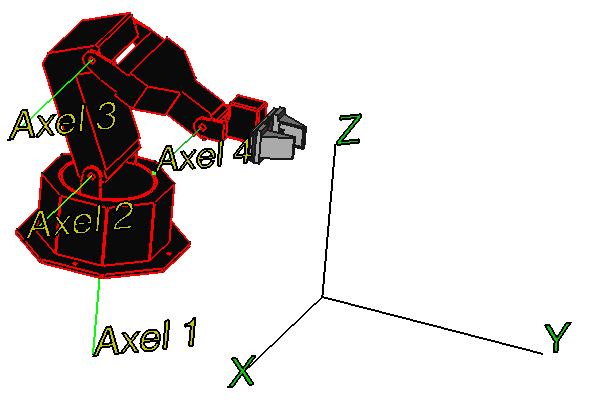
\includegraphics[scale=0.4]{robotaxis}}
\caption{\todo{Kaption}}
\end{figure}

%	\documentclass[10pt,a4paper]{article}
%\usepackage[latin1]{inputenc}
%\usepackage[english]{babel}
%\usepackage{amsmath}
%\usepackage{amsfonts}
%\usepackage{amssymb}
%\usepackage{tikz}
%\title{Gränssnitt för PC}
%\author{Daniel Wassing}
%\begin{document}
	%\maketitle
\section{PC-enhet}
	\subsection{GUI}
	\begin{itemize}
		\item Ska skrivas i Python
		\item Ska kunna skicka följande signaler:
		\begin{enumerate}
			\item motor=L,R (L,R är ints för speed)
			\item arm=X,Y,Z,P,G (Pitch, Grip (allt är ints))
			\item calibrate
			\item status
			\item automotor=M (0/1)
			\item autoarm=A (0/1)
			\item Arm ska EVENTUELLT styras med 2st 2-D kartor, där man kan välja var man går i varje. Förslagsvis att de uppdelas i XY- och XZ-led.
		\end{enumerate}
		\item Ska vara ett GUI (först terminal)
		\item Ska vara en "overhead" för modulen.
		
		%"commando1=X;commando2;commando3=X,Y,Z"
	\end{itemize}
	\pagebreak
	
	\subsection{Modul}
	\begin{itemize}
		\item Ska skrivas i Python
		\item Är "hjärnan" mellan GUI och BT-förbindelse till DAD
		\item Ska ha funktion för att ta emot signal från GUI
		\item Ska ha funktion för att slussa ut en sträng till BT där strängen är en lista på kommandon för vad som ska göras hos DAD (kan vara samma funktion som signalmottagaren)
		\item Strängen ska skickas via en socket-förbindelse. \\
		Se https://wiki.python.org/moin/TcpCommunication för mer info.
	\end{itemize}
	\pagebreak

	\centerline{Figur 1: Flödesschema för PC-modul}
	\centerline{} %empty line
	\centerline{% Graphic for TeX using PGF
% Title: C:\Users\Admin\Pictures\PCflowchart.dia
% Creator: Dia v0.97.2
% CreationDate: Thu Oct 09 11:09:50 2014
% For: Admin
% \usepackage{tikz}
% The following commands are not supported in PSTricks at present
% We define them conditionally, so when they are implemented,
% this pgf file will use them.
\ifx\du\undefined
  \newlength{\du}
\fi
\setlength{\du}{15\unitlength}
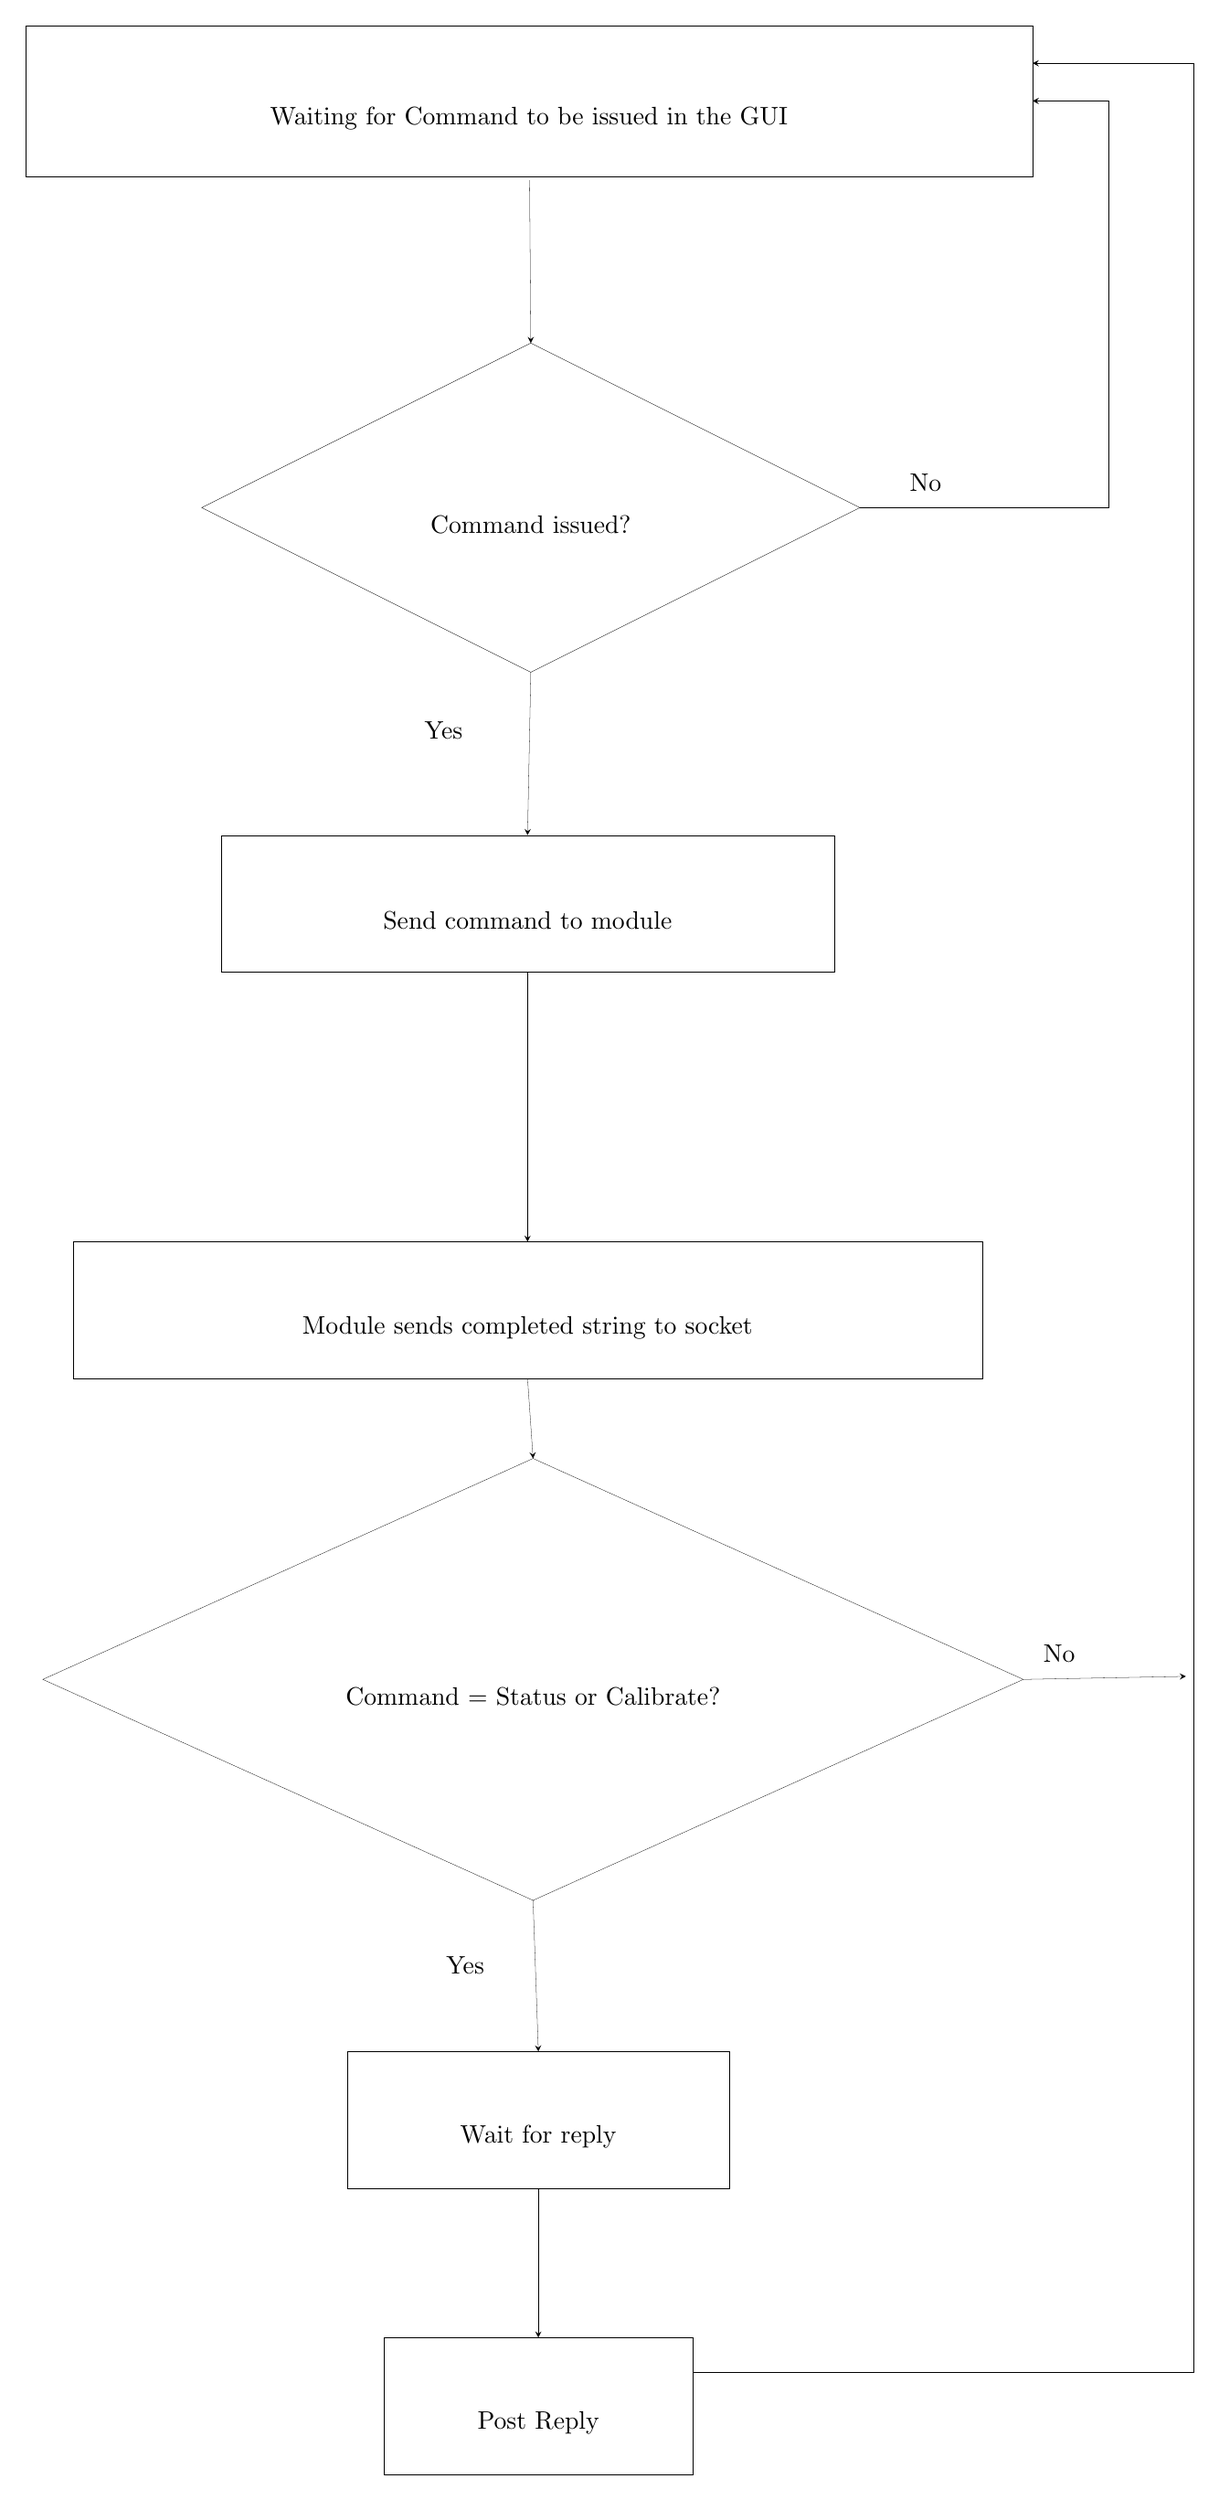
\begin{tikzpicture}
\pgftransformxscale{1.000000}
\pgftransformyscale{-1.000000}
\definecolor{dialinecolor}{rgb}{0.000000, 0.000000, 0.000000}
\pgfsetstrokecolor{dialinecolor}
\definecolor{dialinecolor}{rgb}{1.000000, 1.000000, 1.000000}
\pgfsetfillcolor{dialinecolor}
\definecolor{dialinecolor}{rgb}{1.000000, 1.000000, 1.000000}
\pgfsetfillcolor{dialinecolor}
\fill (5.726250\du,1.700000\du)--(5.726250\du,3.800000\du)--(19.723750\du,3.800000\du)--(19.723750\du,1.700000\du)--cycle;
\pgfsetlinewidth{0.100000\du}
\pgfsetdash{}{0pt}
\pgfsetdash{}{0pt}
\pgfsetmiterjoin
\definecolor{dialinecolor}{rgb}{0.000000, 0.000000, 0.000000}
\pgfsetstrokecolor{dialinecolor}
\draw (5.726250\du,1.700000\du)--(5.726250\du,3.800000\du)--(19.723750\du,3.800000\du)--(19.723750\du,1.700000\du)--cycle;
% setfont left to latex
\definecolor{dialinecolor}{rgb}{0.000000, 0.000000, 0.000000}
\pgfsetstrokecolor{dialinecolor}
\node at (12.725000\du,2.990000\du){Waiting for Command to be issued in the GUI};
\definecolor{dialinecolor}{rgb}{1.000000, 1.000000, 1.000000}
\pgfsetfillcolor{dialinecolor}
\fill (12.750000\du,6.113420\du)--(17.323160\du,8.400000\du)--(12.750000\du,10.686580\du)--(8.176840\du,8.400000\du)--cycle;
\pgfsetlinewidth{0.100000\du}
\pgfsetdash{}{0pt}
\pgfsetdash{}{0pt}
\pgfsetmiterjoin
\definecolor{dialinecolor}{rgb}{0.000000, 0.000000, 0.000000}
\pgfsetstrokecolor{dialinecolor}
\draw (12.750000\du,6.113420\du)--(17.323160\du,8.400000\du)--(12.750000\du,10.686580\du)--(8.176840\du,8.400000\du)--cycle;
% setfont left to latex
\definecolor{dialinecolor}{rgb}{0.000000, 0.000000, 0.000000}
\pgfsetstrokecolor{dialinecolor}
\node at (12.750000\du,8.640000\du){Command issued?};
\pgfsetlinewidth{0.100000\du}
\pgfsetdash{}{0pt}
\pgfsetdash{}{0pt}
\pgfsetmiterjoin
\pgfsetbuttcap
{
\definecolor{dialinecolor}{rgb}{0.000000, 0.000000, 0.000000}
\pgfsetfillcolor{dialinecolor}
% was here!!!
\pgfsetarrowsend{stealth}
{\pgfsetcornersarced{\pgfpoint{0.000000\du}{0.000000\du}}\definecolor{dialinecolor}{rgb}{0.000000, 0.000000, 0.000000}
\pgfsetstrokecolor{dialinecolor}
\draw (17.323200\du,8.400000\du)--(20.773800\du,8.400000\du)--(20.773800\du,2.750000\du)--(19.723800\du,2.750000\du);
}}
% setfont left to latex
\definecolor{dialinecolor}{rgb}{0.000000, 0.000000, 0.000000}
\pgfsetstrokecolor{dialinecolor}
\node[anchor=west] at (17.900000\du,8.050000\du){No};
\pgfsetlinewidth{0.100000\du}
\pgfsetdash{}{0pt}
\pgfsetdash{}{0pt}
\pgfsetbuttcap
{
\definecolor{dialinecolor}{rgb}{0.000000, 0.000000, 0.000000}
\pgfsetfillcolor{dialinecolor}
% was here!!!
\pgfsetarrowsend{stealth}
\definecolor{dialinecolor}{rgb}{0.000000, 0.000000, 0.000000}
\pgfsetstrokecolor{dialinecolor}
\draw (12.733167\du,3.848695\du)--(12.750000\du,6.113420\du);
}
\definecolor{dialinecolor}{rgb}{1.000000, 1.000000, 1.000000}
\pgfsetfillcolor{dialinecolor}
\fill (8.446350\du,12.950000\du)--(8.446350\du,14.850000\du)--(16.963850\du,14.850000\du)--(16.963850\du,12.950000\du)--cycle;
\pgfsetlinewidth{0.100000\du}
\pgfsetdash{}{0pt}
\pgfsetdash{}{0pt}
\pgfsetmiterjoin
\definecolor{dialinecolor}{rgb}{0.000000, 0.000000, 0.000000}
\pgfsetstrokecolor{dialinecolor}
\draw (8.446350\du,12.950000\du)--(8.446350\du,14.850000\du)--(16.963850\du,14.850000\du)--(16.963850\du,12.950000\du)--cycle;
% setfont left to latex
\definecolor{dialinecolor}{rgb}{0.000000, 0.000000, 0.000000}
\pgfsetstrokecolor{dialinecolor}
\node at (12.705100\du,14.140000\du){Send command to module};
\definecolor{dialinecolor}{rgb}{1.000000, 1.000000, 1.000000}
\pgfsetfillcolor{dialinecolor}
\fill (12.781577\du,21.610400\du)--(19.594965\du,24.680018\du)--(12.781577\du,27.749635\du)--(5.968190\du,24.680018\du)--cycle;
\pgfsetlinewidth{0.100000\du}
\pgfsetdash{}{0pt}
\pgfsetdash{}{0pt}
\pgfsetmiterjoin
\definecolor{dialinecolor}{rgb}{0.000000, 0.000000, 0.000000}
\pgfsetstrokecolor{dialinecolor}
\draw (12.781577\du,21.610400\du)--(19.594965\du,24.680018\du)--(12.781577\du,27.749635\du)--(5.968190\du,24.680018\du)--cycle;
% setfont left to latex
\definecolor{dialinecolor}{rgb}{0.000000, 0.000000, 0.000000}
\pgfsetstrokecolor{dialinecolor}
\node at (12.781577\du,24.920018\du){Command = Status or Calibrate?};
\definecolor{dialinecolor}{rgb}{1.000000, 1.000000, 1.000000}
\pgfsetfillcolor{dialinecolor}
\fill (10.202600\du,29.850000\du)--(10.202600\du,31.750000\du)--(15.507600\du,31.750000\du)--(15.507600\du,29.850000\du)--cycle;
\pgfsetlinewidth{0.100000\du}
\pgfsetdash{}{0pt}
\pgfsetdash{}{0pt}
\pgfsetmiterjoin
\definecolor{dialinecolor}{rgb}{0.000000, 0.000000, 0.000000}
\pgfsetstrokecolor{dialinecolor}
\draw (10.202600\du,29.850000\du)--(10.202600\du,31.750000\du)--(15.507600\du,31.750000\du)--(15.507600\du,29.850000\du)--cycle;
% setfont left to latex
\definecolor{dialinecolor}{rgb}{0.000000, 0.000000, 0.000000}
\pgfsetstrokecolor{dialinecolor}
\node at (12.855100\du,31.040000\du){Wait for reply};
\pgfsetlinewidth{0.100000\du}
\pgfsetdash{}{0pt}
\pgfsetdash{}{0pt}
\pgfsetbuttcap
{
\definecolor{dialinecolor}{rgb}{0.000000, 0.000000, 0.000000}
\pgfsetfillcolor{dialinecolor}
% was here!!!
\pgfsetarrowsend{stealth}
\definecolor{dialinecolor}{rgb}{0.000000, 0.000000, 0.000000}
\pgfsetstrokecolor{dialinecolor}
\draw (12.750000\du,10.686600\du)--(12.705100\du,12.950000\du);
}
\pgfsetlinewidth{0.100000\du}
\pgfsetdash{}{0pt}
\pgfsetdash{}{0pt}
\pgfsetbuttcap
{
\definecolor{dialinecolor}{rgb}{0.000000, 0.000000, 0.000000}
\pgfsetfillcolor{dialinecolor}
% was here!!!
\pgfsetarrowsend{stealth}
\definecolor{dialinecolor}{rgb}{0.000000, 0.000000, 0.000000}
\pgfsetstrokecolor{dialinecolor}
\draw (12.705100\du,14.850000\du)--(12.705100\du,18.600000\du);
}
% setfont left to latex
\definecolor{dialinecolor}{rgb}{0.000000, 0.000000, 0.000000}
\pgfsetstrokecolor{dialinecolor}
\node[anchor=west] at (11.155100\du,11.500000\du){Yes};
\pgfsetlinewidth{0.100000\du}
\pgfsetdash{}{0pt}
\pgfsetdash{}{0pt}
\pgfsetbuttcap
{
\definecolor{dialinecolor}{rgb}{0.000000, 0.000000, 0.000000}
\pgfsetfillcolor{dialinecolor}
% was here!!!
\pgfsetarrowsend{stealth}
\definecolor{dialinecolor}{rgb}{0.000000, 0.000000, 0.000000}
\pgfsetstrokecolor{dialinecolor}
\draw (12.781600\du,27.749700\du)--(12.855100\du,29.850000\du);
}
\definecolor{dialinecolor}{rgb}{1.000000, 1.000000, 1.000000}
\pgfsetfillcolor{dialinecolor}
\fill (6.386350\du,18.600000\du)--(6.386350\du,20.500000\du)--(19.023850\du,20.500000\du)--(19.023850\du,18.600000\du)--cycle;
\pgfsetlinewidth{0.100000\du}
\pgfsetdash{}{0pt}
\pgfsetdash{}{0pt}
\pgfsetmiterjoin
\definecolor{dialinecolor}{rgb}{0.000000, 0.000000, 0.000000}
\pgfsetstrokecolor{dialinecolor}
\draw (6.386350\du,18.600000\du)--(6.386350\du,20.500000\du)--(19.023850\du,20.500000\du)--(19.023850\du,18.600000\du)--cycle;
% setfont left to latex
\definecolor{dialinecolor}{rgb}{0.000000, 0.000000, 0.000000}
\pgfsetstrokecolor{dialinecolor}
\node at (12.705100\du,19.790000\du){Module sends completed string to socket};
\pgfsetlinewidth{0.100000\du}
\pgfsetdash{}{0pt}
\pgfsetdash{}{0pt}
\pgfsetbuttcap
{
\definecolor{dialinecolor}{rgb}{0.000000, 0.000000, 0.000000}
\pgfsetfillcolor{dialinecolor}
% was here!!!
\pgfsetarrowsend{stealth}
\definecolor{dialinecolor}{rgb}{0.000000, 0.000000, 0.000000}
\pgfsetstrokecolor{dialinecolor}
\draw (12.705100\du,20.500000\du)--(12.781600\du,21.610400\du);
}
\definecolor{dialinecolor}{rgb}{1.000000, 1.000000, 1.000000}
\pgfsetfillcolor{dialinecolor}
\fill (10.711400\du,33.825000\du)--(10.711400\du,35.725000\du)--(14.998900\du,35.725000\du)--(14.998900\du,33.825000\du)--cycle;
\pgfsetlinewidth{0.100000\du}
\pgfsetdash{}{0pt}
\pgfsetdash{}{0pt}
\pgfsetmiterjoin
\definecolor{dialinecolor}{rgb}{0.000000, 0.000000, 0.000000}
\pgfsetstrokecolor{dialinecolor}
\draw (10.711400\du,33.825000\du)--(10.711400\du,35.725000\du)--(14.998900\du,35.725000\du)--(14.998900\du,33.825000\du)--cycle;
% setfont left to latex
\definecolor{dialinecolor}{rgb}{0.000000, 0.000000, 0.000000}
\pgfsetstrokecolor{dialinecolor}
\node at (12.855150\du,35.015000\du){Post Reply};
\pgfsetlinewidth{0.100000\du}
\pgfsetdash{}{0pt}
\pgfsetdash{}{0pt}
\pgfsetbuttcap
{
\definecolor{dialinecolor}{rgb}{0.000000, 0.000000, 0.000000}
\pgfsetfillcolor{dialinecolor}
% was here!!!
\pgfsetarrowsend{stealth}
\definecolor{dialinecolor}{rgb}{0.000000, 0.000000, 0.000000}
\pgfsetstrokecolor{dialinecolor}
\draw (12.855100\du,31.750000\du)--(12.855100\du,33.825000\du);
}
\pgfsetlinewidth{0.100000\du}
\pgfsetdash{}{0pt}
\pgfsetdash{}{0pt}
\pgfsetmiterjoin
\pgfsetbuttcap
{
\definecolor{dialinecolor}{rgb}{0.000000, 0.000000, 0.000000}
\pgfsetfillcolor{dialinecolor}
% was here!!!
\pgfsetarrowsend{stealth}
{\pgfsetcornersarced{\pgfpoint{0.000000\du}{0.000000\du}}\definecolor{dialinecolor}{rgb}{0.000000, 0.000000, 0.000000}
\pgfsetstrokecolor{dialinecolor}
\draw (14.998900\du,34.300000\du)--(21.955100\du,34.300000\du)--(21.955100\du,2.225000\du)--(19.723800\du,2.225000\du);
}}
\pgfsetlinewidth{0.100000\du}
\pgfsetdash{}{0pt}
\pgfsetdash{}{0pt}
\pgfsetbuttcap
{
\definecolor{dialinecolor}{rgb}{0.000000, 0.000000, 0.000000}
\pgfsetfillcolor{dialinecolor}
% was here!!!
\pgfsetarrowsend{stealth}
\definecolor{dialinecolor}{rgb}{0.000000, 0.000000, 0.000000}
\pgfsetstrokecolor{dialinecolor}
\draw (19.595000\du,24.680000\du)--(21.855100\du,24.637500\du);
}
% setfont left to latex
\definecolor{dialinecolor}{rgb}{0.000000, 0.000000, 0.000000}
\pgfsetstrokecolor{dialinecolor}
\node[anchor=west] at (19.755100\du,24.325000\du){No};
% setfont left to latex
\definecolor{dialinecolor}{rgb}{0.000000, 0.000000, 0.000000}
\pgfsetstrokecolor{dialinecolor}
\node[anchor=west] at (11.455100\du,28.650000\du){Yes};
\end{tikzpicture}
}
	\pagebreak	
	
	\subsection{Fjärrstyrning}
	\begin{itemize}
		\item Ska vara en BT-förbindelse mellan PC och DAD.
		\item Sätts upp via ett PAN (Personal Area Network)
		\item BT-dongel via USB på Beagleboard
		\item BT-support finns redan på PC
	\end{itemize}
%\end{document}

\setcounter{secnumdepth}{5}
\section{Huvudmodul}
Huvudmodulen utför de flesta beräkningar nödvändiga för att roboten ska kunna utföra sina uppgifter. Dessa uppgifter ska huvudmodulen hantera antingen via kommandon från en PC eller helt autonomt. Detta är en kritisk modul då den kommer att utföra många uppgifter. Den behöver inte mycket hårdvara men den kommer innehålla majoriteten av robotens programvara.

\subsection{Hårdvara}
Modulen ska bestå av en enkortsdator av modell Beagleboard. Den har en ARM Cortex-A8 processor som har en klockfrekvens på 1GHz. Denna behöver ett operativsystem för att kunna användas. Den enda hårdvaran som behövs för att kunna använda BB är ett minneskort för operativsystem och en Blåtands-dongel för kommunikationen med PC:n. Kommunikation med sensorenhet och styrenhet sker över SPI.

\subsection{Mjukvara}
Mjukvaran som behövs för att implementera all funktionalitet hos huvudmodulen kommer att vara skriven i programspråket Python. Koden för programmet kommer vara trådbaserad och möjligen objektorienterad. 
\newline
Programmet ska delas in i 3 trådar. Dessa körs kontinuerligt och delar på två trådsäkra listor: sensorvärden och kommandon. I kommandolistan ligger alla argument till tillhörande kommando från PC och i sensorvärden ligger all data från sensorenheten. Listorna kan trådarna antingen läsa eller skriva till (se figur \ref{designspec:huvudmodul-tradar}).

\begin{figure}[h]
\scalebox{0.8}{% Graphic for TeX using PGF
% Title: /home/martin/Downloads/trådar.dia
% Creator: Dia v0.97.2
% CreationDate: Mon Oct  6 14:56:04 2014
% For: martin
% \usepackage{tikz}
% The following commands are not supported in PSTricks at present
% We define them conditionally, so when they are implemented,
% this pgf file will use them.
\ifx\du\undefined
  \newlength{\du}
\fi
\setlength{\du}{15\unitlength}
\begin{tikzpicture}
\pgftransformxscale{1.000000}
\pgftransformyscale{-1.000000}
\definecolor{dialinecolor}{rgb}{0.000000, 0.000000, 0.000000}
\pgfsetstrokecolor{dialinecolor}
\definecolor{dialinecolor}{rgb}{1.000000, 1.000000, 1.000000}
\pgfsetfillcolor{dialinecolor}
\pgfsetlinewidth{0.100000\du}
\pgfsetdash{}{0pt}
\definecolor{dialinecolor}{rgb}{1.000000, 1.000000, 1.000000}
\pgfsetfillcolor{dialinecolor}
\fill (83.362742\du,-37.782161\du)--(83.362742\du,-36.382161\du)--(89.792742\du,-36.382161\du)--(89.792742\du,-37.782161\du)--cycle;
\definecolor{dialinecolor}{rgb}{0.000000, 0.000000, 0.000000}
\pgfsetstrokecolor{dialinecolor}
\draw (83.362742\du,-37.782161\du)--(83.362742\du,-36.382161\du)--(89.792742\du,-36.382161\du)--(89.792742\du,-37.782161\du)--cycle;
% setfont left to latex
\definecolor{dialinecolor}{rgb}{0.000000, 0.000000, 0.000000}
\pgfsetstrokecolor{dialinecolor}
\node at (86.577742\du,-36.832161\du){HUVUD-TRÅD};
\pgfsetlinewidth{0.100000\du}
\pgfsetdash{}{0pt}
\definecolor{dialinecolor}{rgb}{1.000000, 1.000000, 1.000000}
\pgfsetfillcolor{dialinecolor}
\fill (70.982742\du,-37.669161\du)--(70.982742\du,-36.269161\du)--(77.805242\du,-36.269161\du)--(77.805242\du,-37.669161\du)--cycle;
\definecolor{dialinecolor}{rgb}{0.000000, 0.000000, 0.000000}
\pgfsetstrokecolor{dialinecolor}
\draw (70.982742\du,-37.669161\du)--(70.982742\du,-36.269161\du)--(77.805242\du,-36.269161\du)--(77.805242\du,-37.669161\du)--cycle;
% setfont left to latex
\definecolor{dialinecolor}{rgb}{0.000000, 0.000000, 0.000000}
\pgfsetstrokecolor{dialinecolor}
\node at (74.393992\du,-36.719161\du){SENSOR-TRÅD};
\pgfsetlinewidth{0.100000\du}
\pgfsetdash{}{0pt}
\definecolor{dialinecolor}{rgb}{1.000000, 1.000000, 1.000000}
\pgfsetfillcolor{dialinecolor}
\fill (76.282742\du,-33.369161\du)--(76.282742\du,-31.969161\du)--(82.932742\du,-31.969161\du)--(82.932742\du,-33.369161\du)--cycle;
\definecolor{dialinecolor}{rgb}{0.000000, 0.000000, 0.000000}
\pgfsetstrokecolor{dialinecolor}
\draw (76.282742\du,-33.369161\du)--(76.282742\du,-31.969161\du)--(82.932742\du,-31.969161\du)--(82.932742\du,-33.369161\du)--cycle;
% setfont left to latex
\definecolor{dialinecolor}{rgb}{0.000000, 0.000000, 0.000000}
\pgfsetstrokecolor{dialinecolor}
\node at (79.607742\du,-32.419161\du){sensorvärden};
\definecolor{dialinecolor}{rgb}{1.000000, 1.000000, 1.000000}
\pgfsetfillcolor{dialinecolor}
\fill (76.282742\du,-31.969161\du)--(76.282742\du,-31.569161\du)--(82.932742\du,-31.569161\du)--(82.932742\du,-31.969161\du)--cycle;
\definecolor{dialinecolor}{rgb}{0.000000, 0.000000, 0.000000}
\pgfsetstrokecolor{dialinecolor}
\draw (76.282742\du,-31.969161\du)--(76.282742\du,-31.569161\du)--(82.932742\du,-31.569161\du)--(82.932742\du,-31.969161\du)--cycle;
\definecolor{dialinecolor}{rgb}{1.000000, 1.000000, 1.000000}
\pgfsetfillcolor{dialinecolor}
\fill (76.282742\du,-31.569161\du)--(76.282742\du,-31.169161\du)--(82.932742\du,-31.169161\du)--(82.932742\du,-31.569161\du)--cycle;
\definecolor{dialinecolor}{rgb}{0.000000, 0.000000, 0.000000}
\pgfsetstrokecolor{dialinecolor}
\draw (76.282742\du,-31.569161\du)--(76.282742\du,-31.169161\du)--(82.932742\du,-31.169161\du)--(82.932742\du,-31.569161\du)--cycle;
\pgfsetlinewidth{0.100000\du}
\pgfsetdash{}{0pt}
\definecolor{dialinecolor}{rgb}{1.000000, 1.000000, 1.000000}
\pgfsetfillcolor{dialinecolor}
\fill (88.732742\du,-33.369161\du)--(88.732742\du,-31.969161\du)--(94.760242\du,-31.969161\du)--(94.760242\du,-33.369161\du)--cycle;
\definecolor{dialinecolor}{rgb}{0.000000, 0.000000, 0.000000}
\pgfsetstrokecolor{dialinecolor}
\draw (88.732742\du,-33.369161\du)--(88.732742\du,-31.969161\du)--(94.760242\du,-31.969161\du)--(94.760242\du,-33.369161\du)--cycle;
% setfont left to latex
\definecolor{dialinecolor}{rgb}{0.000000, 0.000000, 0.000000}
\pgfsetstrokecolor{dialinecolor}
\node at (91.746492\du,-32.419161\du){kommandon};
\definecolor{dialinecolor}{rgb}{1.000000, 1.000000, 1.000000}
\pgfsetfillcolor{dialinecolor}
\fill (88.732742\du,-31.969161\du)--(88.732742\du,-31.569161\du)--(94.760242\du,-31.569161\du)--(94.760242\du,-31.969161\du)--cycle;
\definecolor{dialinecolor}{rgb}{0.000000, 0.000000, 0.000000}
\pgfsetstrokecolor{dialinecolor}
\draw (88.732742\du,-31.969161\du)--(88.732742\du,-31.569161\du)--(94.760242\du,-31.569161\du)--(94.760242\du,-31.969161\du)--cycle;
\definecolor{dialinecolor}{rgb}{1.000000, 1.000000, 1.000000}
\pgfsetfillcolor{dialinecolor}
\fill (88.732742\du,-31.569161\du)--(88.732742\du,-31.169161\du)--(94.760242\du,-31.169161\du)--(94.760242\du,-31.569161\du)--cycle;
\definecolor{dialinecolor}{rgb}{0.000000, 0.000000, 0.000000}
\pgfsetstrokecolor{dialinecolor}
\draw (88.732742\du,-31.569161\du)--(88.732742\du,-31.169161\du)--(94.760242\du,-31.169161\du)--(94.760242\du,-31.569161\du)--cycle;
\pgfsetlinewidth{0.100000\du}
\pgfsetdash{}{0pt}
\definecolor{dialinecolor}{rgb}{1.000000, 1.000000, 1.000000}
\pgfsetfillcolor{dialinecolor}
\fill (97.282742\du,-37.657161\du)--(97.282742\du,-36.257161\du)--(101.635242\du,-36.257161\du)--(101.635242\du,-37.657161\du)--cycle;
\definecolor{dialinecolor}{rgb}{0.000000, 0.000000, 0.000000}
\pgfsetstrokecolor{dialinecolor}
\draw (97.282742\du,-37.657161\du)--(97.282742\du,-36.257161\du)--(101.635242\du,-36.257161\du)--(101.635242\du,-37.657161\du)--cycle;
% setfont left to latex
\definecolor{dialinecolor}{rgb}{0.000000, 0.000000, 0.000000}
\pgfsetstrokecolor{dialinecolor}
\node at (99.458992\du,-36.707161\du){PC-TRÅD};
\pgfsetlinewidth{0.100000\du}
\pgfsetdash{}{0pt}
\pgfsetdash{}{0pt}
\pgfsetbuttcap
{
\definecolor{dialinecolor}{rgb}{0.000000, 0.000000, 0.000000}
\pgfsetfillcolor{dialinecolor}
% was here!!!
\pgfsetarrowsstart{stealth}
\pgfsetarrowsend{stealth}
\definecolor{dialinecolor}{rgb}{0.000000, 0.000000, 0.000000}
\pgfsetstrokecolor{dialinecolor}
\draw (81.072842\du,-33.469161\du)--(85.291242\du,-36.382161\du);
}
\pgfsetlinewidth{0.100000\du}
\pgfsetdash{}{0pt}
\pgfsetdash{}{0pt}
\pgfsetbuttcap
{
\definecolor{dialinecolor}{rgb}{0.000000, 0.000000, 0.000000}
\pgfsetfillcolor{dialinecolor}
% was here!!!
\pgfsetarrowsend{stealth}
\definecolor{dialinecolor}{rgb}{0.000000, 0.000000, 0.000000}
\pgfsetstrokecolor{dialinecolor}
\draw (75.225188\du,-36.219869\du)--(78.331671\du,-33.419491\du);
}
\pgfsetlinewidth{0.100000\du}
\pgfsetdash{}{0pt}
\pgfsetdash{}{0pt}
\pgfsetmiterjoin
\pgfsetbuttcap
{
\definecolor{dialinecolor}{rgb}{0.000000, 0.000000, 0.000000}
\pgfsetfillcolor{dialinecolor}
% was here!!!
\pgfsetarrowsend{stealth}
{\pgfsetcornersarced{\pgfpoint{0.000000\du}{0.000000\du}}\definecolor{dialinecolor}{rgb}{0.000000, 0.000000, 0.000000}
\pgfsetstrokecolor{dialinecolor}
\draw (79.607742\du,-31.169161\du)--(79.607742\du,-27.644161\du)--(99.458992\du,-27.644161\du)--(99.458992\du,-36.257161\du);
}}
\pgfsetlinewidth{0.100000\du}
\pgfsetdash{}{0pt}
\pgfsetdash{}{0pt}
\pgfsetbuttcap
{
\definecolor{dialinecolor}{rgb}{0.000000, 0.000000, 0.000000}
\pgfsetfillcolor{dialinecolor}
% was here!!!
\pgfsetarrowsstart{to}
\pgfsetarrowsend{stealth}
\definecolor{dialinecolor}{rgb}{0.000000, 0.000000, 0.000000}
\pgfsetstrokecolor{dialinecolor}
\draw (93.732742\du,-33.444161\du)--(99.458992\du,-36.257161\du);
}
\pgfsetlinewidth{0.100000\du}
\pgfsetdash{}{0pt}
\pgfsetdash{}{0pt}
\pgfsetbuttcap
{
\definecolor{dialinecolor}{rgb}{0.000000, 0.000000, 0.000000}
\pgfsetfillcolor{dialinecolor}
% was here!!!
\pgfsetarrowsstart{stealth}
\definecolor{dialinecolor}{rgb}{0.000000, 0.000000, 0.000000}
\pgfsetstrokecolor{dialinecolor}
\draw (87.782742\du,-36.282161\du)--(91.746492\du,-33.369161\du);
}
\pgfsetlinewidth{0.100000\du}
\pgfsetdash{}{0pt}
\pgfsetdash{}{0pt}
\pgfsetmiterjoin
\pgfsetbuttcap
{
\definecolor{dialinecolor}{rgb}{0.000000, 0.000000, 0.000000}
\pgfsetfillcolor{dialinecolor}
% was here!!!
\pgfsetarrowsstart{stealth}
{\pgfsetcornersarced{\pgfpoint{0.000000\du}{0.000000\du}}\definecolor{dialinecolor}{rgb}{0.000000, 0.000000, 0.000000}
\pgfsetstrokecolor{dialinecolor}
\draw (74.393992\du,-37.669161\du)--(74.393992\du,-42.382161\du)--(92.582742\du,-42.382161\du)--(92.582742\du,-33.432161\du);
}}
\end{tikzpicture}
}
\caption{Trådarna och listorna de delar på} \label{designspec:huvudmodul-tradar}
\end{figure}

Det som behövs göras på BB innan den kan börja användas är:
\begin{itemize}
\item Installera Angstrom operativsystem
\item uppdatera operativsystem
\item installera python
\item konfigurera spi
\item patcha kärnan för att stödja SPI
\item installera git
\item installera eclipse/emacs
\item installera blåtandsmodulen
\item sätta upp ett PAN
\end{itemize}

\subsubsection{Huvudtråden}
I huvudtråden ligger huvudloopen för programmet. Den börjar med att läsa värdet från kommandolistan där manuell eller autonomt läge avgörs och kallar på respektive funktion. Användaren ska alltså kunna växla mellan dessa lägen när denne vill (mellan varje iteration av huvudloopen). Figur \ref{designspec:huvudmodul-huvudtrad} illustrerar programflödet.
\paragraph{Autonomt läge}
\leavevmode
\newline
\newline
Här ska kod för autonom aktivitet hos systemet ligga. Sensorvärdeslistan behöver läsas av varje iteration för att avgöra om systemet befinner sig vid en av- eller upplockningsstation samt om systemet behöver regleras. Om systemet befinner sig vid en upplockningsstation behöver vi läsa av kommandolistan för att få argument om att styra armen. Om systemet befinner sig vid en avplockningsstation ska systemet låsa sig tills paket är avsläppt.
\newline 
Om systemet inte befinner sig vid en av- eller upplockningsstation skickas värden till styrenheten att köra roboten framåt. Dessa värden beräknas i slutet av programmet med regleringsalgoritmen utifrån linjesensordata från sensorvärdeslistan. 
\paragraph{Manuellt läge}
\leavevmode
\newline
\newline
I manuellt läge läses argumenten från kommandolistan av, tolkar dessa och skickar vidare lämpliga värden till styrenheten.

\begin{figure}[h]
\centering
\scalebox{0.6}{% Graphic for TeX using PGF
% Title: /home/mumsaren/Dokument/TSEA29/Dokumentation/huvudtråd.dia
% Creator: Dia v0.97.2
% CreationDate: Thu Oct  9 17:00:07 2014
% For: mumsaren
% \usepackage{tikz}
% The following commands are not supported in PSTricks at present
% We define them conditionally, so when they are implemented,
% this pgf file will use them.
\ifx\du\undefined
  \newlength{\du}
\fi
\setlength{\du}{15\unitlength}
\begin{tikzpicture}
\pgftransformxscale{1.000000}
\pgftransformyscale{-1.000000}
\definecolor{dialinecolor}{rgb}{0.000000, 0.000000, 0.000000}
\pgfsetstrokecolor{dialinecolor}
\definecolor{dialinecolor}{rgb}{1.000000, 1.000000, 1.000000}
\pgfsetfillcolor{dialinecolor}
\definecolor{dialinecolor}{rgb}{1.000000, 1.000000, 1.000000}
\pgfsetfillcolor{dialinecolor}
\fill (18.338750\du,11.550000\du)--(18.338750\du,13.450000\du)--(25.861250\du,13.450000\du)--(25.861250\du,11.550000\du)--cycle;
\pgfsetlinewidth{0.100000\du}
\pgfsetdash{}{0pt}
\pgfsetdash{}{0pt}
\pgfsetmiterjoin
\definecolor{dialinecolor}{rgb}{0.000000, 0.000000, 0.000000}
\pgfsetstrokecolor{dialinecolor}
\draw (18.338750\du,11.550000\du)--(18.338750\du,13.450000\du)--(25.861250\du,13.450000\du)--(25.861250\du,11.550000\du)--cycle;
% setfont left to latex
\definecolor{dialinecolor}{rgb}{0.000000, 0.000000, 0.000000}
\pgfsetstrokecolor{dialinecolor}
\node at (22.100000\du,12.695000\du){läs kommandolistan};
\definecolor{dialinecolor}{rgb}{1.000000, 1.000000, 1.000000}
\pgfsetfillcolor{dialinecolor}
\fill (22.100000\du,16.366545\du)--(24.966910\du,17.800000\du)--(22.100000\du,19.233455\du)--(19.233090\du,17.800000\du)--cycle;
\pgfsetlinewidth{0.100000\du}
\pgfsetdash{}{0pt}
\pgfsetdash{}{0pt}
\pgfsetmiterjoin
\definecolor{dialinecolor}{rgb}{0.000000, 0.000000, 0.000000}
\pgfsetstrokecolor{dialinecolor}
\draw (22.100000\du,16.366545\du)--(24.966910\du,17.800000\du)--(22.100000\du,19.233455\du)--(19.233090\du,17.800000\du)--cycle;
% setfont left to latex
\definecolor{dialinecolor}{rgb}{0.000000, 0.000000, 0.000000}
\pgfsetstrokecolor{dialinecolor}
\node at (22.100000\du,17.995000\du){läge?};
\pgfsetlinewidth{0.100000\du}
\pgfsetdash{}{0pt}
\pgfsetdash{}{0pt}
\pgfsetbuttcap
{
\definecolor{dialinecolor}{rgb}{0.000000, 0.000000, 0.000000}
\pgfsetfillcolor{dialinecolor}
% was here!!!
\pgfsetarrowsend{stealth}
\definecolor{dialinecolor}{rgb}{0.000000, 0.000000, 0.000000}
\pgfsetstrokecolor{dialinecolor}
\draw (22.100000\du,13.450000\du)--(22.100000\du,16.366545\du);
}
\pgfsetlinewidth{0.100000\du}
\pgfsetdash{}{0pt}
\pgfsetdash{}{0pt}
\pgfsetmiterjoin
\pgfsetbuttcap
{
\definecolor{dialinecolor}{rgb}{0.000000, 0.000000, 0.000000}
\pgfsetfillcolor{dialinecolor}
% was here!!!
\pgfsetarrowsstart{stealth}
{\pgfsetcornersarced{\pgfpoint{0.000000\du}{0.000000\du}}\definecolor{dialinecolor}{rgb}{0.000000, 0.000000, 0.000000}
\pgfsetstrokecolor{dialinecolor}
\draw (18.338750\du,12.500000\du)--(17.288750\du,12.500000\du)--(17.288750\du,17.800000\du)--(19.233090\du,17.800000\du);
}}
\pgfsetlinewidth{0.100000\du}
\pgfsetdash{}{0pt}
\pgfsetdash{}{0pt}
\pgfsetbuttcap
{
\definecolor{dialinecolor}{rgb}{0.000000, 0.000000, 0.000000}
\pgfsetfillcolor{dialinecolor}
% was here!!!
\pgfsetarrowsend{stealth}
\definecolor{dialinecolor}{rgb}{0.000000, 0.000000, 0.000000}
\pgfsetstrokecolor{dialinecolor}
\draw (24.966910\du,17.800000\du)--(28.730590\du,17.850000\du);
}
% setfont left to latex
\definecolor{dialinecolor}{rgb}{0.000000, 0.000000, 0.000000}
\pgfsetstrokecolor{dialinecolor}
\node[anchor=west] at (25.400000\du,17.000000\du){manuellt};
\definecolor{dialinecolor}{rgb}{1.000000, 1.000000, 1.000000}
\pgfsetfillcolor{dialinecolor}
\fill (28.905000\du,16.900000\du)--(28.905000\du,18.800000\du)--(36.795000\du,18.800000\du)--(36.795000\du,16.900000\du)--cycle;
\pgfsetlinewidth{0.100000\du}
\pgfsetdash{}{0pt}
\pgfsetdash{}{0pt}
\pgfsetmiterjoin
\definecolor{dialinecolor}{rgb}{0.000000, 0.000000, 0.000000}
\pgfsetstrokecolor{dialinecolor}
\draw (28.905000\du,16.900000\du)--(28.905000\du,18.800000\du)--(36.795000\du,18.800000\du)--(36.795000\du,16.900000\du)--cycle;
% setfont left to latex
\definecolor{dialinecolor}{rgb}{0.000000, 0.000000, 0.000000}
\pgfsetstrokecolor{dialinecolor}
\node at (32.850000\du,18.045000\du){Utför kommandon};
\pgfsetlinewidth{0.100000\du}
\pgfsetdash{}{0pt}
\pgfsetdash{}{0pt}
\pgfsetmiterjoin
\pgfsetbuttcap
{
\definecolor{dialinecolor}{rgb}{0.000000, 0.000000, 0.000000}
\pgfsetfillcolor{dialinecolor}
% was here!!!
\pgfsetarrowsstart{stealth}
{\pgfsetcornersarced{\pgfpoint{0.000000\du}{0.000000\du}}\definecolor{dialinecolor}{rgb}{0.000000, 0.000000, 0.000000}
\pgfsetstrokecolor{dialinecolor}
\draw (25.861250\du,12.500000\du)--(32.850000\du,12.500000\du)--(32.850000\du,16.900000\du);
}}
\definecolor{dialinecolor}{rgb}{1.000000, 1.000000, 1.000000}
\pgfsetfillcolor{dialinecolor}
\fill (22.050000\du,22.125295\du)--(25.774410\du,23.987500\du)--(22.050000\du,25.849705\du)--(18.325590\du,23.987500\du)--cycle;
\pgfsetlinewidth{0.100000\du}
\pgfsetdash{}{0pt}
\pgfsetdash{}{0pt}
\pgfsetmiterjoin
\definecolor{dialinecolor}{rgb}{0.000000, 0.000000, 0.000000}
\pgfsetstrokecolor{dialinecolor}
\draw (22.050000\du,22.125295\du)--(25.774410\du,23.987500\du)--(22.050000\du,25.849705\du)--(18.325590\du,23.987500\du)--cycle;
% setfont left to latex
\definecolor{dialinecolor}{rgb}{0.000000, 0.000000, 0.000000}
\pgfsetstrokecolor{dialinecolor}
\node at (22.050000\du,24.182500\du){styra arm?};
\pgfsetlinewidth{0.100000\du}
\pgfsetdash{}{0pt}
\pgfsetdash{}{0pt}
\pgfsetbuttcap
{
\definecolor{dialinecolor}{rgb}{0.000000, 0.000000, 0.000000}
\pgfsetfillcolor{dialinecolor}
% was here!!!
\pgfsetarrowsend{stealth}
\definecolor{dialinecolor}{rgb}{0.000000, 0.000000, 0.000000}
\pgfsetstrokecolor{dialinecolor}
\draw (22.100000\du,19.233455\du)--(22.050000\du,22.125295\du);
}
% setfont left to latex
\definecolor{dialinecolor}{rgb}{0.000000, 0.000000, 0.000000}
\pgfsetstrokecolor{dialinecolor}
\node[anchor=west] at (22.700000\du,20.687500\du){autonomt};
\definecolor{dialinecolor}{rgb}{1.000000, 1.000000, 1.000000}
\pgfsetfillcolor{dialinecolor}
\fill (32.806947\du,21.099512\du)--(36.298304\du,24.009611\du)--(32.806947\du,26.919711\du)--(29.315590\du,24.009611\du)--cycle;
\pgfsetlinewidth{0.100000\du}
\pgfsetdash{}{0pt}
\pgfsetdash{}{0pt}
\pgfsetmiterjoin
\definecolor{dialinecolor}{rgb}{0.000000, 0.000000, 0.000000}
\pgfsetstrokecolor{dialinecolor}
\draw (32.806947\du,21.099512\du)--(36.298304\du,24.009611\du)--(32.806947\du,26.919711\du)--(29.315590\du,24.009611\du)--cycle;
% setfont left to latex
\definecolor{dialinecolor}{rgb}{0.000000, 0.000000, 0.000000}
\pgfsetstrokecolor{dialinecolor}
\node at (32.806947\du,24.204611\du){upplockning?};
\pgfsetlinewidth{0.100000\du}
\pgfsetdash{}{0pt}
\pgfsetdash{}{0pt}
\pgfsetbuttcap
{
\definecolor{dialinecolor}{rgb}{0.000000, 0.000000, 0.000000}
\pgfsetfillcolor{dialinecolor}
% was here!!!
\pgfsetarrowsend{stealth}
\definecolor{dialinecolor}{rgb}{0.000000, 0.000000, 0.000000}
\pgfsetstrokecolor{dialinecolor}
\draw (25.774410\du,23.987500\du)--(29.315590\du,24.009611\du);
}
% setfont left to latex
\definecolor{dialinecolor}{rgb}{0.000000, 0.000000, 0.000000}
\pgfsetstrokecolor{dialinecolor}
\node[anchor=west] at (32.850000\du,17.850000\du){};
% setfont left to latex
\definecolor{dialinecolor}{rgb}{0.000000, 0.000000, 0.000000}
\pgfsetstrokecolor{dialinecolor}
\node[anchor=west] at (26.800000\du,23.387500\du){nej};
\pgfsetlinewidth{0.100000\du}
\pgfsetdash{}{0pt}
\pgfsetdash{}{0pt}
\pgfsetbuttcap
{
\definecolor{dialinecolor}{rgb}{0.000000, 0.000000, 0.000000}
\pgfsetfillcolor{dialinecolor}
% was here!!!
\definecolor{dialinecolor}{rgb}{0.000000, 0.000000, 0.000000}
\pgfsetstrokecolor{dialinecolor}
\draw (36.298304\du,24.009611\du)--(40.150000\du,23.987500\du);
}
% setfont left to latex
\definecolor{dialinecolor}{rgb}{0.000000, 0.000000, 0.000000}
\pgfsetstrokecolor{dialinecolor}
\node[anchor=west] at (37.850000\du,23.387500\du){ja};
\definecolor{dialinecolor}{rgb}{1.000000, 1.000000, 1.000000}
\pgfsetfillcolor{dialinecolor}
\fill (32.804150\du,29.967795\du)--(36.222710\du,32.982309\du)--(32.804150\du,35.996823\du)--(29.385590\du,32.982309\du)--cycle;
\pgfsetlinewidth{0.100000\du}
\pgfsetdash{}{0pt}
\pgfsetdash{}{0pt}
\pgfsetmiterjoin
\definecolor{dialinecolor}{rgb}{0.000000, 0.000000, 0.000000}
\pgfsetstrokecolor{dialinecolor}
\draw (32.804150\du,29.967795\du)--(36.222710\du,32.982309\du)--(32.804150\du,35.996823\du)--(29.385590\du,32.982309\du)--cycle;
% setfont left to latex
\definecolor{dialinecolor}{rgb}{0.000000, 0.000000, 0.000000}
\pgfsetstrokecolor{dialinecolor}
\node at (32.804150\du,33.177309\du){avplockning?};
\pgfsetlinewidth{0.100000\du}
\pgfsetdash{}{0pt}
\pgfsetdash{}{0pt}
\pgfsetbuttcap
{
\definecolor{dialinecolor}{rgb}{0.000000, 0.000000, 0.000000}
\pgfsetfillcolor{dialinecolor}
% was here!!!
\pgfsetarrowsend{stealth}
\definecolor{dialinecolor}{rgb}{0.000000, 0.000000, 0.000000}
\pgfsetstrokecolor{dialinecolor}
\draw (32.806947\du,26.919711\du)--(32.804150\du,29.967795\du);
}
% setfont left to latex
\definecolor{dialinecolor}{rgb}{0.000000, 0.000000, 0.000000}
\pgfsetstrokecolor{dialinecolor}
\node[anchor=west] at (33.300000\du,28.225000\du){nej};
\definecolor{dialinecolor}{rgb}{1.000000, 1.000000, 1.000000}
\pgfsetfillcolor{dialinecolor}
\fill (39.907500\du,32.075000\du)--(39.907500\du,33.975000\du)--(45.492500\du,33.975000\du)--(45.492500\du,32.075000\du)--cycle;
\pgfsetlinewidth{0.100000\du}
\pgfsetdash{}{0pt}
\pgfsetdash{}{0pt}
\pgfsetmiterjoin
\definecolor{dialinecolor}{rgb}{0.000000, 0.000000, 0.000000}
\pgfsetstrokecolor{dialinecolor}
\draw (39.907500\du,32.075000\du)--(39.907500\du,33.975000\du)--(45.492500\du,33.975000\du)--(45.492500\du,32.075000\du)--cycle;
% setfont left to latex
\definecolor{dialinecolor}{rgb}{0.000000, 0.000000, 0.000000}
\pgfsetstrokecolor{dialinecolor}
\node at (42.700000\du,33.220000\du){sätt ner paket};
\pgfsetlinewidth{0.100000\du}
\pgfsetdash{}{0pt}
\pgfsetdash{}{0pt}
\pgfsetbuttcap
{
\definecolor{dialinecolor}{rgb}{0.000000, 0.000000, 0.000000}
\pgfsetfillcolor{dialinecolor}
% was here!!!
\pgfsetarrowsend{stealth}
\definecolor{dialinecolor}{rgb}{0.000000, 0.000000, 0.000000}
\pgfsetstrokecolor{dialinecolor}
\draw (36.222710\du,32.982309\du)--(39.907500\du,33.025000\du);
}
% setfont left to latex
\definecolor{dialinecolor}{rgb}{0.000000, 0.000000, 0.000000}
\pgfsetstrokecolor{dialinecolor}
\node[anchor=west] at (37.550000\du,32.425000\du){ja};
\pgfsetlinewidth{0.100000\du}
\pgfsetdash{}{0pt}
\pgfsetdash{}{0pt}
\pgfsetmiterjoin
\pgfsetbuttcap
{
\definecolor{dialinecolor}{rgb}{0.000000, 0.000000, 0.000000}
\pgfsetfillcolor{dialinecolor}
% was here!!!
{\pgfsetcornersarced{\pgfpoint{0.000000\du}{0.000000\du}}\definecolor{dialinecolor}{rgb}{0.000000, 0.000000, 0.000000}
\pgfsetstrokecolor{dialinecolor}
\draw (42.700000\du,32.075000\du)--(42.700000\du,28.006250\du)--(40.100000\du,28.006250\du)--(40.100000\du,23.937500\du);
}}
\definecolor{dialinecolor}{rgb}{1.000000, 1.000000, 1.000000}
\pgfsetfillcolor{dialinecolor}
\fill (11.552500\du,23.037500\du)--(11.552500\du,24.937500\du)--(15.347500\du,24.937500\du)--(15.347500\du,23.037500\du)--cycle;
\pgfsetlinewidth{0.100000\du}
\pgfsetdash{}{0pt}
\pgfsetdash{}{0pt}
\pgfsetmiterjoin
\definecolor{dialinecolor}{rgb}{0.000000, 0.000000, 0.000000}
\pgfsetstrokecolor{dialinecolor}
\draw (11.552500\du,23.037500\du)--(11.552500\du,24.937500\du)--(15.347500\du,24.937500\du)--(15.347500\du,23.037500\du)--cycle;
% setfont left to latex
\definecolor{dialinecolor}{rgb}{0.000000, 0.000000, 0.000000}
\pgfsetstrokecolor{dialinecolor}
\node at (13.450000\du,24.182500\du){styr arm};
\pgfsetlinewidth{0.100000\du}
\pgfsetdash{}{0pt}
\pgfsetdash{}{0pt}
\pgfsetbuttcap
{
\definecolor{dialinecolor}{rgb}{0.000000, 0.000000, 0.000000}
\pgfsetfillcolor{dialinecolor}
% was here!!!
\pgfsetarrowsend{stealth}
\definecolor{dialinecolor}{rgb}{0.000000, 0.000000, 0.000000}
\pgfsetstrokecolor{dialinecolor}
\draw (18.325590\du,23.987500\du)--(15.347500\du,23.987500\du);
}
% setfont left to latex
\definecolor{dialinecolor}{rgb}{0.000000, 0.000000, 0.000000}
\pgfsetstrokecolor{dialinecolor}
\node[anchor=west] at (16.700000\du,23.387500\du){ja};
\pgfsetlinewidth{0.100000\du}
\pgfsetdash{}{0pt}
\pgfsetdash{}{0pt}
\pgfsetmiterjoin
\pgfsetbuttcap
{
\definecolor{dialinecolor}{rgb}{0.000000, 0.000000, 0.000000}
\pgfsetfillcolor{dialinecolor}
% was here!!!
{\pgfsetcornersarced{\pgfpoint{0.000000\du}{0.000000\du}}\definecolor{dialinecolor}{rgb}{0.000000, 0.000000, 0.000000}
\pgfsetstrokecolor{dialinecolor}
\draw (13.450000\du,23.037500\du)--(13.450000\du,17.812500\du)--(17.300000\du,17.812500\du)--(17.300000\du,12.587500\du);
}}
% setfont left to latex
\definecolor{dialinecolor}{rgb}{0.000000, 0.000000, 0.000000}
\pgfsetstrokecolor{dialinecolor}
\node[anchor=west] at (17.550000\du,17.387500\du){inget};
\definecolor{dialinecolor}{rgb}{1.000000, 1.000000, 1.000000}
\pgfsetfillcolor{dialinecolor}
\fill (18.970000\du,32.075000\du)--(18.970000\du,33.975000\du)--(25.030000\du,33.975000\du)--(25.030000\du,32.075000\du)--cycle;
\pgfsetlinewidth{0.100000\du}
\pgfsetdash{}{0pt}
\pgfsetdash{}{0pt}
\pgfsetmiterjoin
\definecolor{dialinecolor}{rgb}{0.000000, 0.000000, 0.000000}
\pgfsetstrokecolor{dialinecolor}
\draw (18.970000\du,32.075000\du)--(18.970000\du,33.975000\du)--(25.030000\du,33.975000\du)--(25.030000\du,32.075000\du)--cycle;
% setfont left to latex
\definecolor{dialinecolor}{rgb}{0.000000, 0.000000, 0.000000}
\pgfsetstrokecolor{dialinecolor}
\node at (22.000000\du,33.220000\du){läs sensorlistan};
\pgfsetlinewidth{0.100000\du}
\pgfsetdash{}{0pt}
\pgfsetdash{}{0pt}
\pgfsetbuttcap
{
\definecolor{dialinecolor}{rgb}{0.000000, 0.000000, 0.000000}
\pgfsetfillcolor{dialinecolor}
% was here!!!
\pgfsetarrowsend{stealth}
\definecolor{dialinecolor}{rgb}{0.000000, 0.000000, 0.000000}
\pgfsetstrokecolor{dialinecolor}
\draw (29.385590\du,32.982309\du)--(25.030000\du,33.025000\du);
}
% setfont left to latex
\definecolor{dialinecolor}{rgb}{0.000000, 0.000000, 0.000000}
\pgfsetstrokecolor{dialinecolor}
\node[anchor=west] at (26.700000\du,32.325000\du){nej};
\definecolor{dialinecolor}{rgb}{1.000000, 1.000000, 1.000000}
\pgfsetfillcolor{dialinecolor}
\fill (13.928750\du,36.875000\du)--(13.928750\du,38.775000\du)--(30.071250\du,38.775000\du)--(30.071250\du,36.875000\du)--cycle;
\pgfsetlinewidth{0.100000\du}
\pgfsetdash{}{0pt}
\pgfsetdash{}{0pt}
\pgfsetmiterjoin
\definecolor{dialinecolor}{rgb}{0.000000, 0.000000, 0.000000}
\pgfsetstrokecolor{dialinecolor}
\draw (13.928750\du,36.875000\du)--(13.928750\du,38.775000\du)--(30.071250\du,38.775000\du)--(30.071250\du,36.875000\du)--cycle;
% setfont left to latex
\definecolor{dialinecolor}{rgb}{0.000000, 0.000000, 0.000000}
\pgfsetstrokecolor{dialinecolor}
\node at (22.000000\du,38.020000\du){sätt variablerna upplockning och avplockning};
\pgfsetlinewidth{0.100000\du}
\pgfsetdash{}{0pt}
\pgfsetdash{}{0pt}
\pgfsetbuttcap
{
\definecolor{dialinecolor}{rgb}{0.000000, 0.000000, 0.000000}
\pgfsetfillcolor{dialinecolor}
% was here!!!
\pgfsetarrowsend{stealth}
\definecolor{dialinecolor}{rgb}{0.000000, 0.000000, 0.000000}
\pgfsetstrokecolor{dialinecolor}
\draw (22.000000\du,33.975000\du)--(22.000000\du,36.875000\du);
}
\definecolor{dialinecolor}{rgb}{1.000000, 1.000000, 1.000000}
\pgfsetfillcolor{dialinecolor}
\fill (20.311250\du,41.312500\du)--(20.311250\du,43.212500\du)--(23.688750\du,43.212500\du)--(23.688750\du,41.312500\du)--cycle;
\pgfsetlinewidth{0.100000\du}
\pgfsetdash{}{0pt}
\pgfsetdash{}{0pt}
\pgfsetmiterjoin
\definecolor{dialinecolor}{rgb}{0.000000, 0.000000, 0.000000}
\pgfsetstrokecolor{dialinecolor}
\draw (20.311250\du,41.312500\du)--(20.311250\du,43.212500\du)--(23.688750\du,43.212500\du)--(23.688750\du,41.312500\du)--cycle;
% setfont left to latex
\definecolor{dialinecolor}{rgb}{0.000000, 0.000000, 0.000000}
\pgfsetstrokecolor{dialinecolor}
\node at (22.000000\du,42.457500\du){reglera};
\pgfsetlinewidth{0.100000\du}
\pgfsetdash{}{0pt}
\pgfsetdash{}{0pt}
\pgfsetbuttcap
{
\definecolor{dialinecolor}{rgb}{0.000000, 0.000000, 0.000000}
\pgfsetfillcolor{dialinecolor}
% was here!!!
\pgfsetarrowsend{stealth}
\definecolor{dialinecolor}{rgb}{0.000000, 0.000000, 0.000000}
\pgfsetstrokecolor{dialinecolor}
\draw (22.000000\du,38.775000\du)--(22.000000\du,41.312500\du);
}
\definecolor{dialinecolor}{rgb}{1.000000, 1.000000, 1.000000}
\pgfsetfillcolor{dialinecolor}
\fill (19.775000\du,46.200000\du)--(19.775000\du,48.100000\du)--(24.225000\du,48.100000\du)--(24.225000\du,46.200000\du)--cycle;
\pgfsetlinewidth{0.100000\du}
\pgfsetdash{}{0pt}
\pgfsetdash{}{0pt}
\pgfsetmiterjoin
\definecolor{dialinecolor}{rgb}{0.000000, 0.000000, 0.000000}
\pgfsetstrokecolor{dialinecolor}
\draw (19.775000\du,46.200000\du)--(19.775000\du,48.100000\du)--(24.225000\du,48.100000\du)--(24.225000\du,46.200000\du)--cycle;
% setfont left to latex
\definecolor{dialinecolor}{rgb}{0.000000, 0.000000, 0.000000}
\pgfsetstrokecolor{dialinecolor}
\node at (22.000000\du,47.345000\du){kör framåt};
% setfont left to latex
\definecolor{dialinecolor}{rgb}{0.000000, 0.000000, 0.000000}
\pgfsetstrokecolor{dialinecolor}
\node[anchor=west] at (22.000000\du,47.150000\du){};
% setfont left to latex
\definecolor{dialinecolor}{rgb}{0.000000, 0.000000, 0.000000}
\pgfsetstrokecolor{dialinecolor}
\node[anchor=west] at (22.000000\du,47.150000\du){};
\pgfsetlinewidth{0.100000\du}
\pgfsetdash{}{0pt}
\pgfsetdash{}{0pt}
\pgfsetbuttcap
{
\definecolor{dialinecolor}{rgb}{0.000000, 0.000000, 0.000000}
\pgfsetfillcolor{dialinecolor}
% was here!!!
\pgfsetarrowsend{stealth}
\definecolor{dialinecolor}{rgb}{0.000000, 0.000000, 0.000000}
\pgfsetstrokecolor{dialinecolor}
\draw (22.000000\du,43.212500\du)--(22.000000\du,46.200000\du);
}
\pgfsetlinewidth{0.100000\du}
\pgfsetdash{}{0pt}
\pgfsetdash{}{0pt}
\pgfsetmiterjoin
\pgfsetbuttcap
{
\definecolor{dialinecolor}{rgb}{0.000000, 0.000000, 0.000000}
\pgfsetfillcolor{dialinecolor}
% was here!!!
{\pgfsetcornersarced{\pgfpoint{0.000000\du}{0.000000\du}}\definecolor{dialinecolor}{rgb}{0.000000, 0.000000, 0.000000}
\pgfsetstrokecolor{dialinecolor}
\draw (17.350000\du,12.562500\du)--(8.750000\du,12.562500\du)--(8.750000\du,47.150000\du)--(19.775000\du,47.150000\du);
}}
\pgfsetlinewidth{0.100000\du}
\pgfsetdash{}{0pt}
\pgfsetdash{}{0pt}
\pgfsetmiterjoin
\pgfsetbuttcap
{
\definecolor{dialinecolor}{rgb}{0.000000, 0.000000, 0.000000}
\pgfsetfillcolor{dialinecolor}
% was here!!!
{\pgfsetcornersarced{\pgfpoint{0.000000\du}{0.000000\du}}\definecolor{dialinecolor}{rgb}{0.000000, 0.000000, 0.000000}
\pgfsetstrokecolor{dialinecolor}
\draw (40.150000\du,24.000000\du)--(40.150000\du,15.962500\du)--(32.850000\du,15.962500\du)--(32.850000\du,14.062500\du);
}}
\end{tikzpicture}
}
\caption{Flödesschema för huvudtråden} \label{designspec:huvudmodul-huvudtrad}
\end{figure}

\subsubsection{Sensortråden}
Sensortrådens uppgift är att uppdatera sensorvärdeslistan med fräscha värden från sensorenheten.

\subsubsection{PC-tråden}
PC-tråden delar upp strängen med data från PC och lägger endast in argumenten från de olika kommandona i kommandolistan.

\subsection{Reglering}
För att undvika att roboten hackar sig fram och istället rör sig med smidiga rörelser så ska motorns styrsignaler regleras med en tidsdiskret PD-regulator. En PID regulator är onödig då vi inte har något stående fel i teorin. Om roboten är mitt på linjen och står rakt så kommer felet vara noll. I praktiken kommer det inte vara så då roboten troligtvis inte kommer stå rakt på linjen och motorerna kommer säkert åka i olika hastigheter. Dock så blir en PD-regulator tillräckligt bra. En annan anledning till att inte ha med I-delen är att det är svårt att implementera det bra i ett tidsdiskret system. 
\begin{itemize}
\item $e[n]$ Är felet vid sampling n
\item $e[n-1]$ Är felet vid sampling n-1
\item $u[n]$ är styrsignalen till motorerna
\item $K_{P}$ är en konstant för den proportionella delen av regleringen
\item $K_{D}$ är en konstant för den deriverande delen av regleringen
\item $\Delta T$ är tiden mellan sampling n och n-1
 
\end{itemize}
 $$ u[n] = K_P*e[n] + K_D\frac{e[n]-e[n-1]}{\Delta T}$$
 Roboten är begränsade av hårdvaran hur ofta den kan läsa av data från reflexsensorna. Enligt handledaren är en uppdatering på 25 Hertz en rimlig nivå. Så $\Delta T$ kommer vara 40ms. \todo{Se över detta stycke. "handledaren" rimlig referens?}

 \subsection{Styrning av arm}
 Omvandlingen från x,y,z koordinater till vinklar för armens servons kommer att ske i huvudmodulen då det är en rätt krävande operation. Tanken är att när roboten stannar vid en station så ska användaren kunna styra robotens arm med en joystick eller från tangentbordet. När användaren beordrar armen att röra sig framåt så ska armen röra sig i positiv y-led i förhållande till roboten. När användaren beodrar roboten att styra åt höger så ska armens ändpunkt röra sig i positivt x-led i förhållande till roboten.
 \newline
 \begin{figure}[h]
 \centerline{% Graphic for TeX using PGF
% Title: /home/martin/Diagram1.dia
% Creator: Dia v0.97.2
% CreationDate: Sun Oct 12 18:13:42 2014
% For: martin
% \usepackage{tikz}
% The following commands are not supported in PSTricks at present
% We define them conditionally, so when they are implemented,
% this pgf file will use them.
\ifx\du\undefined
  \newlength{\du}
\fi
\setlength{\du}{15\unitlength}
\begin{tikzpicture}
\pgftransformxscale{1.000000}
\pgftransformyscale{-1.000000}
\definecolor{dialinecolor}{rgb}{0.000000, 0.000000, 0.000000}
\pgfsetstrokecolor{dialinecolor}
\definecolor{dialinecolor}{rgb}{1.000000, 1.000000, 1.000000}
\pgfsetfillcolor{dialinecolor}
\pgfsetlinewidth{0.100000\du}
\pgfsetdash{}{0pt}
\pgfsetdash{}{0pt}
\pgfsetmiterjoin
\definecolor{dialinecolor}{rgb}{1.000000, 1.000000, 1.000000}
\pgfsetfillcolor{dialinecolor}
\fill (3.300000\du,-2.250000\du)--(3.300000\du,4.212500\du)--(8.950000\du,4.212500\du)--(8.950000\du,-2.250000\du)--cycle;
\definecolor{dialinecolor}{rgb}{0.000000, 0.000000, 0.000000}
\pgfsetstrokecolor{dialinecolor}
\draw (3.300000\du,-2.250000\du)--(3.300000\du,4.212500\du)--(8.950000\du,4.212500\du)--(8.950000\du,-2.250000\du)--cycle;
\pgfsetlinewidth{0.100000\du}
\pgfsetdash{}{0pt}
\pgfsetdash{}{0pt}
\pgfsetbuttcap
\pgfsetmiterjoin
\pgfsetlinewidth{0.100000\du}
\pgfsetbuttcap
\pgfsetmiterjoin
\pgfsetdash{}{0pt}
\definecolor{dialinecolor}{rgb}{1.000000, 1.000000, 1.000000}
\pgfsetfillcolor{dialinecolor}
\pgfpathellipse{\pgfpoint{6.137500\du}{0.787500\du}}{\pgfpoint{1.537500\du}{0\du}}{\pgfpoint{0\du}{1.537500\du}}
\pgfusepath{fill}
\definecolor{dialinecolor}{rgb}{0.000000, 0.000000, 0.000000}
\pgfsetstrokecolor{dialinecolor}
\pgfpathellipse{\pgfpoint{6.137500\du}{0.787500\du}}{\pgfpoint{1.537500\du}{0\du}}{\pgfpoint{0\du}{1.537500\du}}
\pgfusepath{stroke}
\pgfsetbuttcap
\pgfsetmiterjoin
\pgfsetdash{}{0pt}
\definecolor{dialinecolor}{rgb}{0.000000, 0.000000, 0.000000}
\pgfsetstrokecolor{dialinecolor}
\pgfpathellipse{\pgfpoint{6.137500\du}{0.787500\du}}{\pgfpoint{1.537500\du}{0\du}}{\pgfpoint{0\du}{1.537500\du}}
\pgfusepath{stroke}
\pgfsetlinewidth{0.100000\du}
\pgfsetdash{}{0pt}
\pgfsetdash{}{0pt}
\pgfsetbuttcap
{
\definecolor{dialinecolor}{rgb}{0.000000, 0.000000, 0.000000}
\pgfsetfillcolor{dialinecolor}
% was here!!!
\definecolor{dialinecolor}{rgb}{0.000000, 0.000000, 0.000000}
\pgfsetstrokecolor{dialinecolor}
\draw (7.231647\du,-0.360394\du)--(9.700000\du,-2.950000\du);
}
\pgfsetlinewidth{0.100000\du}
\pgfsetdash{}{0pt}
\pgfsetdash{}{0pt}
\pgfsetbuttcap
{
\definecolor{dialinecolor}{rgb}{0.000000, 0.000000, 0.000000}
\pgfsetfillcolor{dialinecolor}
% was here!!!
\pgfsetarrowsend{to}
\definecolor{dialinecolor}{rgb}{0.000000, 0.000000, 0.000000}
\pgfsetstrokecolor{dialinecolor}
\draw (9.850000\du,-3.000000\du)--(14.300000\du,-2.950000\du);
}
\pgfsetlinewidth{0.100000\du}
\pgfsetdash{}{0pt}
\pgfsetdash{}{0pt}
\pgfsetbuttcap
{
\definecolor{dialinecolor}{rgb}{0.000000, 0.000000, 0.000000}
\pgfsetfillcolor{dialinecolor}
% was here!!!
\pgfsetarrowsend{to}
\definecolor{dialinecolor}{rgb}{0.000000, 0.000000, 0.000000}
\pgfsetstrokecolor{dialinecolor}
\draw (9.750000\du,-3.187500\du)--(9.700000\du,-7.637500\du);
}
% setfont left to latex
\definecolor{dialinecolor}{rgb}{0.000000, 0.000000, 0.000000}
\pgfsetstrokecolor{dialinecolor}
\node[anchor=west] at (14.650000\du,-2.787500\du){X-led};
% setfont left to latex
\definecolor{dialinecolor}{rgb}{0.000000, 0.000000, 0.000000}
\pgfsetstrokecolor{dialinecolor}
\node[anchor=west] at (9.700000\du,-7.737500\du){Y-led};
\end{tikzpicture}
}
 \caption{\todo{Kaption}}
 \end{figure}
 \begin{figure}[h]
\centerline{% Graphic for TeX using PGF
% Title: /home/martin/wdawd.dia
% Creator: Dia v0.97.2
% CreationDate: Sun Oct 12 20:26:39 2014
% For: martin
% \usepackage{tikz}
% The following commands are not supported in PSTricks at present
% We define them conditionally, so when they are implemented,
% this pgf file will use them.
\ifx\du\undefined
  \newlength{\du}
\fi
\setlength{\du}{15\unitlength}
\begin{tikzpicture}
\pgftransformxscale{1.000000}
\pgftransformyscale{-1.000000}
\definecolor{dialinecolor}{rgb}{0.000000, 0.000000, 0.000000}
\pgfsetstrokecolor{dialinecolor}
\definecolor{dialinecolor}{rgb}{1.000000, 1.000000, 1.000000}
\pgfsetfillcolor{dialinecolor}
\pgfsetlinewidth{0.100000\du}
\pgfsetdash{}{0pt}
\pgfsetdash{}{0pt}
\pgfsetbuttcap
{
\definecolor{dialinecolor}{rgb}{0.000000, 0.000000, 0.000000}
\pgfsetfillcolor{dialinecolor}
% was here!!!
\definecolor{dialinecolor}{rgb}{0.000000, 0.000000, 0.000000}
\pgfsetstrokecolor{dialinecolor}
\draw (3.650000\du,5.762500\du)--(7.900000\du,-1.587500\du);
}
\pgfsetlinewidth{0.100000\du}
\pgfsetdash{}{0pt}
\pgfsetdash{}{0pt}
\pgfsetbuttcap
{
\definecolor{dialinecolor}{rgb}{0.000000, 0.000000, 0.000000}
\pgfsetfillcolor{dialinecolor}
% was here!!!
\definecolor{dialinecolor}{rgb}{0.000000, 0.000000, 0.000000}
\pgfsetstrokecolor{dialinecolor}
\draw (7.850000\du,-1.537500\du)--(17.900000\du,-1.487500\du);
}
\pgfsetlinewidth{0.100000\du}
\pgfsetdash{}{0pt}
\pgfsetdash{}{0pt}
\pgfsetbuttcap
{
\definecolor{dialinecolor}{rgb}{0.000000, 0.000000, 0.000000}
\pgfsetfillcolor{dialinecolor}
% was here!!!
\definecolor{dialinecolor}{rgb}{0.000000, 0.000000, 0.000000}
\pgfsetstrokecolor{dialinecolor}
\draw (17.850000\du,-1.437500\du)--(20.900000\du,2.962500\du);
}
\pgfsetlinewidth{0.100000\du}
\pgfsetdash{{1.000000\du}{1.000000\du}}{0\du}
\pgfsetdash{{1.000000\du}{1.000000\du}}{0\du}
\pgfsetbuttcap
{
\definecolor{dialinecolor}{rgb}{0.000000, 0.000000, 0.000000}
\pgfsetfillcolor{dialinecolor}
% was here!!!
\definecolor{dialinecolor}{rgb}{0.000000, 0.000000, 0.000000}
\pgfsetstrokecolor{dialinecolor}
\draw (3.600000\du,6.162500\du)--(3.600000\du,-7.087500\du);
}
\pgfsetlinewidth{0.100000\du}
\pgfsetdash{{1.000000\du}{1.000000\du}}{0\du}
\pgfsetdash{{1.000000\du}{1.000000\du}}{0\du}
\pgfsetbuttcap
{
\definecolor{dialinecolor}{rgb}{0.000000, 0.000000, 0.000000}
\pgfsetfillcolor{dialinecolor}
% was here!!!
\definecolor{dialinecolor}{rgb}{0.000000, 0.000000, 0.000000}
\pgfsetstrokecolor{dialinecolor}
\draw (3.700000\du,6.212500\du)--(27.500000\du,6.062500\du);
}
\pgfsetlinewidth{0.100000\du}
\pgfsetdash{}{0pt}
\pgfsetdash{}{0pt}
\pgfsetbuttcap
{
\definecolor{dialinecolor}{rgb}{0.000000, 0.000000, 0.000000}
\pgfsetfillcolor{dialinecolor}
% was here!!!
\definecolor{dialinecolor}{rgb}{0.000000, 0.000000, 0.000000}
\pgfsetstrokecolor{dialinecolor}
\pgfpathmoveto{\pgfpoint{6.049937\du}{6.212702\du}}
\pgfpatharc{18}{-65}{2.110604\du and 2.110604\du}
\pgfusepath{stroke}
}
\pgfsetlinewidth{0.100000\du}
\pgfsetdash{}{0pt}
\pgfsetdash{}{0pt}
\pgfsetbuttcap
{
\definecolor{dialinecolor}{rgb}{0.000000, 0.000000, 0.000000}
\pgfsetfillcolor{dialinecolor}
% was here!!!
\definecolor{dialinecolor}{rgb}{0.000000, 0.000000, 0.000000}
\pgfsetstrokecolor{dialinecolor}
\pgfpathmoveto{\pgfpoint{6.949854\du}{0.062444\du}}
\pgfpatharc{112}{9}{2.148827\du and 2.148827\du}
\pgfusepath{stroke}
}
\pgfsetlinewidth{0.100000\du}
\pgfsetdash{}{0pt}
\pgfsetdash{}{0pt}
\pgfsetbuttcap
{
\definecolor{dialinecolor}{rgb}{0.000000, 0.000000, 0.000000}
\pgfsetfillcolor{dialinecolor}
% was here!!!
\definecolor{dialinecolor}{rgb}{0.000000, 0.000000, 0.000000}
\pgfsetstrokecolor{dialinecolor}
\pgfpathmoveto{\pgfpoint{16.550022\du}{-1.537549\du}}
\pgfpatharc{205}{42}{1.170625\du and 1.170625\du}
\pgfusepath{stroke}
}
\pgfsetlinewidth{0.100000\du}
\pgfsetdash{{1.000000\du}{1.000000\du}}{0\du}
\pgfsetdash{{1.000000\du}{1.000000\du}}{0\du}
\pgfsetbuttcap
{
\definecolor{dialinecolor}{rgb}{0.000000, 0.000000, 0.000000}
\pgfsetfillcolor{dialinecolor}
% was here!!!
\definecolor{dialinecolor}{rgb}{0.000000, 0.000000, 0.000000}
\pgfsetstrokecolor{dialinecolor}
\draw (18.200000\du,2.962500\du)--(27.950000\du,2.912500\du);
}
\pgfsetlinewidth{0.100000\du}
\pgfsetdash{}{0pt}
\pgfsetdash{}{0pt}
\pgfsetbuttcap
{
\definecolor{dialinecolor}{rgb}{0.000000, 0.000000, 0.000000}
\pgfsetfillcolor{dialinecolor}
% was here!!!
\definecolor{dialinecolor}{rgb}{0.000000, 0.000000, 0.000000}
\pgfsetstrokecolor{dialinecolor}
\pgfpathmoveto{\pgfpoint{19.950016\du}{1.812506\du}}
\pgfpatharc{292}{159}{0.849480\du and 0.849480\du}
\pgfusepath{stroke}
}
% setfont left to latex
\definecolor{dialinecolor}{rgb}{0.000000, 0.000000, 0.000000}
\pgfsetstrokecolor{dialinecolor}
\node[anchor=west] at (0.500000\du,6.112500\du){P0=(0,0)};
% setfont left to latex
\definecolor{dialinecolor}{rgb}{0.000000, 0.000000, 0.000000}
\pgfsetstrokecolor{dialinecolor}
\node[anchor=west] at (5.650000\du,4.062500\du){A1};
% setfont left to latex
\definecolor{dialinecolor}{rgb}{0.000000, 0.000000, 0.000000}
\pgfsetstrokecolor{dialinecolor}
\node[anchor=west] at (8.900000\du,0.862500\du){A2};
% setfont left to latex
\definecolor{dialinecolor}{rgb}{0.000000, 0.000000, 0.000000}
\pgfsetstrokecolor{dialinecolor}
\node[anchor=west] at (16.350000\du,0.762500\du){A3};
% setfont left to latex
\definecolor{dialinecolor}{rgb}{0.000000, 0.000000, 0.000000}
\pgfsetstrokecolor{dialinecolor}
\node[anchor=west] at (14.800000\du,2.562500\du){};
% setfont left to latex
\definecolor{dialinecolor}{rgb}{0.000000, 0.000000, 0.000000}
\pgfsetstrokecolor{dialinecolor}
\node[anchor=west] at (18.150000\du,1.812500\du){};
% setfont left to latex
\definecolor{dialinecolor}{rgb}{0.000000, 0.000000, 0.000000}
\pgfsetstrokecolor{dialinecolor}
\node[anchor=west] at (17.850000\du,2.062500\du){A4};
% setfont left to latex
\definecolor{dialinecolor}{rgb}{0.000000, 0.000000, 0.000000}
\pgfsetstrokecolor{dialinecolor}
\node[anchor=west] at (4.850000\du,1.162500\du){L1};
% setfont left to latex
\definecolor{dialinecolor}{rgb}{0.000000, 0.000000, 0.000000}
\pgfsetstrokecolor{dialinecolor}
\node[anchor=west] at (12.600000\du,-2.287500\du){L2};
% setfont left to latex
\definecolor{dialinecolor}{rgb}{0.000000, 0.000000, 0.000000}
\pgfsetstrokecolor{dialinecolor}
\node[anchor=west] at (20.050000\du,0.362500\du){L3};
% setfont left to latex
\definecolor{dialinecolor}{rgb}{0.000000, 0.000000, 0.000000}
\pgfsetstrokecolor{dialinecolor}
\node[anchor=west] at (7.100000\du,-2.337500\du){P1=(W1,Z1)};
% setfont left to latex
\definecolor{dialinecolor}{rgb}{0.000000, 0.000000, 0.000000}
\pgfsetstrokecolor{dialinecolor}
\node[anchor=west] at (18.175000\du,-2.337500\du){P2=(W2,Z2)};
% setfont left to latex
\definecolor{dialinecolor}{rgb}{0.000000, 0.000000, 0.000000}
\pgfsetstrokecolor{dialinecolor}
\node[anchor=west] at (20.825000\du,3.912500\du){P3=(W,Z)};
% setfont left to latex
\definecolor{dialinecolor}{rgb}{0.000000, 0.000000, 0.000000}
\pgfsetstrokecolor{dialinecolor}
\node[anchor=west] at (20.925000\du,-2.637500\du){};
\pgfsetlinewidth{0.100000\du}
\pgfsetdash{}{0pt}
\pgfsetdash{}{0pt}
\pgfsetbuttcap
{
\definecolor{dialinecolor}{rgb}{0.000000, 0.000000, 0.000000}
\pgfsetfillcolor{dialinecolor}
% was here!!!
\definecolor{dialinecolor}{rgb}{0.000000, 0.000000, 0.000000}
\pgfsetstrokecolor{dialinecolor}
\draw (3.675000\du,6.212500\du)--(17.725000\du,-1.487500\du);
}
% setfont left to latex
\definecolor{dialinecolor}{rgb}{0.000000, 0.000000, 0.000000}
\pgfsetstrokecolor{dialinecolor}
\node[anchor=west] at (11.775000\du,2.762500\du){HL};
% setfont left to latex
\definecolor{dialinecolor}{rgb}{0.000000, 0.000000, 0.000000}
\pgfsetstrokecolor{dialinecolor}
\node[anchor=west] at (3.225000\du,-8.087500\du){z};
% setfont left to latex
\definecolor{dialinecolor}{rgb}{0.000000, 0.000000, 0.000000}
\pgfsetstrokecolor{dialinecolor}
\node[anchor=west] at (27.125000\du,6.062500\du){w};
\pgfsetlinewidth{0.100000\du}
\pgfsetdash{}{0pt}
\pgfsetdash{}{0pt}
\pgfsetbuttcap
{
\definecolor{dialinecolor}{rgb}{0.000000, 0.000000, 0.000000}
\pgfsetfillcolor{dialinecolor}
% was here!!!
\definecolor{dialinecolor}{rgb}{0.000000, 0.000000, 0.000000}
\pgfsetstrokecolor{dialinecolor}
\pgfpathmoveto{\pgfpoint{8.425000\du}{6.212503\du}}
\pgfpatharc{358}{321}{3.739603\du and 3.739603\du}
\pgfusepath{stroke}
}
% setfont left to latex
\definecolor{dialinecolor}{rgb}{0.000000, 0.000000, 0.000000}
\pgfsetstrokecolor{dialinecolor}
\node[anchor=west] at (8.825000\du,4.762500\du){HA};
\end{tikzpicture}
}
\caption{\todo{Kaption}}
\end{figure}
\newline
 För att detta ska vara möjligt så behöver vi använda lite trionometri. Omvandlingen sker på följande sätt:
Antag att roboten start i: $$X,Y,Z,GR=0,0,0,\pi/2$$
Där GR(GripRadian) är vilken vinkel "handen" har till z-axeln.\newline
Vi omvandlar:$$ X,Y,Z,GR\rightarrow A,W,Z,GR$$ 
Där A är armens vinkel mot positiva x-axel och W är armens utsträckning.
$$A=tan^-1(\dfrac{Y}{X}) $$
$$W=\sqrt{X^2+Y^2}$$
Genom denna omvandlingen så kan vi göra om detta till ett 2D problem istället för ett 3D problem. Vi får in X,Y,Z,GR och ställer in robotens vinkel mot x-axelns positiva del och sedan ser vi till att roboten bara har rätt utsträckning och höjd.
$$P_4=(W,Z)$$
$$P_0=(0,0)$$
$$W_2=W-cos(GR)*L_3$$
$$Z_2=Z-sin(GR)*L_3$$
$$H_L=\sqrt{W_2^2+Z_2^2}$$
$$H_A=tan^-1(\dfrac{Z_2}{W_2})$$
Cosinussatsen ger:
$$A_1=cos^-1(\dfrac{L_1^2+H_L^2-L_2^2}{2*L_1*H_L})+H_A$$
$$W_1=cos(A_1)*L_1$$
$$Z_1=sin(A_1)*L_1$$
$$A_2=tan^-1(\dfrac{Z_2-Z_1}{W_2-W_1})-A_1$$
$$A_3=GR-D_2-D_3$$

Då har vi alla vinklar vi behöver. Sedan är det upp till styrenheten att omvandla dessa vinklar till positioner på servona på armen.
Beräkningarna har simulerats i ett eget python-program:
\begin{figure}[h]
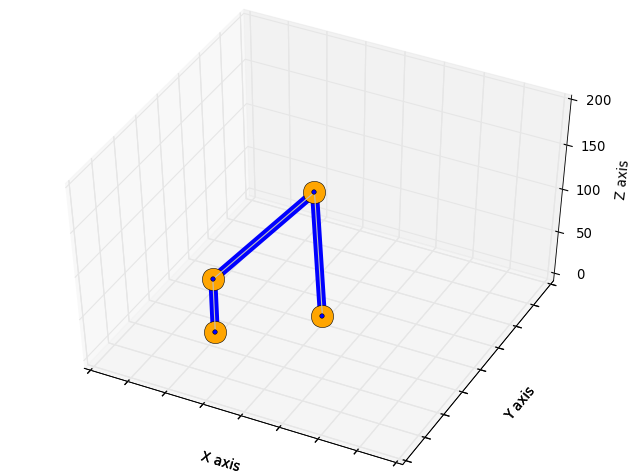
\includegraphics[scale=0.6]{simulator}
\caption{\todo{Kaption}}
\end{figure}
\subsection{hårdvara som behövs}
\begin{itemize}
\item Beagleboard-xm (finns i vanheden)
\item Blåtandsdongel Belkin f8t016(vi har en)
\item Nivåomvandlare Ti TXB0108 ("http://www.electrokit.com/nivaomvandlare-8-kanaler.50717")
\item Minneskort (Om det inte finns i vanheden så beställ från elfa )
\item Wifidongel för utveckling på den (vi har en)
\end{itemize}


%\documentclass[a4paper,11pt]{article}
%\usepackage[a4paper]{}
%\usepackage[utf8]{inputenc}
%\usepackage{listings}
%\usepackage{graphicx}
%\begin{document}

\section{Sensorenhet}
Sensorenheten har till uppgift att läsa in data från robotens sensorer, tolka den och vidarebefodra den till huvudenheten. En reflexsensormodul används för att roboten skall kunna hålla sig på banan. För att kunna detektera paket kommer roboten ha en avståndssensor på vardera sida. \\

\begin{figure}[h]
\center
\scalebox{0.9}{% Graphic for TeX using PGF
% Title: /home/kebabdjuret/Documents/skola/tsea29/gloria/dokumentation/designspecifikation/sensorenhet-blockschema.dia
% Creator: Dia v0.97.2
% CreationDate: Thu Oct  9 14:42:10 2014
% For: kebabdjuret
% \usepackage{tikz}
% The following commands are not supported in PSTricks at present
% We define them conditionally, so when they are implemented,
% this pgf file will use them.
\ifx\du\undefined
  \newlength{\du}
\fi
\setlength{\du}{15\unitlength}
\begin{tikzpicture}
\pgftransformxscale{1.000000}
\pgftransformyscale{-1.000000}
\definecolor{dialinecolor}{rgb}{0.000000, 0.000000, 0.000000}
\pgfsetstrokecolor{dialinecolor}
\definecolor{dialinecolor}{rgb}{1.000000, 1.000000, 1.000000}
\pgfsetfillcolor{dialinecolor}
\pgfsetlinewidth{0.100000\du}
\pgfsetdash{}{0pt}
\pgfsetdash{}{0pt}
\pgfsetmiterjoin
\definecolor{dialinecolor}{rgb}{1.000000, 1.000000, 1.000000}
\pgfsetfillcolor{dialinecolor}
\fill (15.427300\du,9.486540\du)--(15.427300\du,17.645911\du)--(20.127300\du,17.645911\du)--(20.127300\du,9.486540\du)--cycle;
\definecolor{dialinecolor}{rgb}{0.000000, 0.000000, 0.000000}
\pgfsetstrokecolor{dialinecolor}
\draw (15.427300\du,9.486540\du)--(15.427300\du,17.645911\du)--(20.127300\du,17.645911\du)--(20.127300\du,9.486540\du)--cycle;
\pgfsetlinewidth{0.100000\du}
\pgfsetdash{}{0pt}
\pgfsetdash{}{0pt}
\pgfsetmiterjoin
\definecolor{dialinecolor}{rgb}{1.000000, 1.000000, 1.000000}
\pgfsetfillcolor{dialinecolor}
\fill (25.040900\du,10.114600\du)--(25.040900\du,12.022980\du)--(33.816769\du,12.022980\du)--(33.816769\du,10.114600\du)--cycle;
\definecolor{dialinecolor}{rgb}{0.000000, 0.000000, 0.000000}
\pgfsetstrokecolor{dialinecolor}
\draw (25.040900\du,10.114600\du)--(25.040900\du,12.022980\du)--(33.816769\du,12.022980\du)--(33.816769\du,10.114600\du)--cycle;
\pgfsetlinewidth{0.100000\du}
\pgfsetdash{}{0pt}
\pgfsetdash{}{0pt}
\pgfsetmiterjoin
\definecolor{dialinecolor}{rgb}{1.000000, 1.000000, 1.000000}
\pgfsetfillcolor{dialinecolor}
\fill (25.039100\du,12.551500\du)--(25.039100\du,14.459880\du)--(33.816769\du,14.459880\du)--(33.816769\du,12.551500\du)--cycle;
\definecolor{dialinecolor}{rgb}{0.000000, 0.000000, 0.000000}
\pgfsetstrokecolor{dialinecolor}
\draw (25.039100\du,12.551500\du)--(25.039100\du,14.459880\du)--(33.816769\du,14.459880\du)--(33.816769\du,12.551500\du)--cycle;
\pgfsetlinewidth{0.100000\du}
\pgfsetdash{}{0pt}
\pgfsetdash{}{0pt}
\pgfsetbuttcap
{
\definecolor{dialinecolor}{rgb}{0.000000, 0.000000, 0.000000}
\pgfsetfillcolor{dialinecolor}
% was here!!!
\pgfsetarrowsend{to}
\definecolor{dialinecolor}{rgb}{0.000000, 0.000000, 0.000000}
\pgfsetstrokecolor{dialinecolor}
\draw (25.040900\du,11.068790\du)--(20.106300\du,11.102900\du);
}
\pgfsetlinewidth{0.100000\du}
\pgfsetdash{}{0pt}
\pgfsetdash{}{0pt}
\pgfsetbuttcap
{
\definecolor{dialinecolor}{rgb}{0.000000, 0.000000, 0.000000}
\pgfsetfillcolor{dialinecolor}
% was here!!!
\pgfsetarrowsend{to}
\definecolor{dialinecolor}{rgb}{0.000000, 0.000000, 0.000000}
\pgfsetstrokecolor{dialinecolor}
\draw (25.039100\du,13.505690\du)--(20.077600\du,13.540100\du);
}
% setfont left to latex
\definecolor{dialinecolor}{rgb}{0.000000, 0.000000, 0.000000}
\pgfsetstrokecolor{dialinecolor}
\node[anchor=west] at (17.189200\du,13.801900\du){AVR};
\pgfsetlinewidth{0.100000\du}
\pgfsetdash{}{0pt}
\pgfsetdash{}{0pt}
\pgfsetbuttcap
{
\definecolor{dialinecolor}{rgb}{0.000000, 0.000000, 0.000000}
\pgfsetfillcolor{dialinecolor}
% was here!!!
\pgfsetarrowsstart{to}
\pgfsetarrowsend{to}
\definecolor{dialinecolor}{rgb}{0.000000, 0.000000, 0.000000}
\pgfsetstrokecolor{dialinecolor}
\draw (11.216500\du,13.588400\du)--(15.427300\du,13.566200\du);
}
\pgfsetlinewidth{0.100000\du}
\pgfsetdash{}{0pt}
\pgfsetdash{}{0pt}
\pgfsetmiterjoin
\definecolor{dialinecolor}{rgb}{1.000000, 1.000000, 1.000000}
\pgfsetfillcolor{dialinecolor}
\fill (6.691550\du,13.088400\du)--(6.691550\du,14.088391\du)--(11.216510\du,14.088391\du)--(11.216510\du,13.088400\du)--cycle;
\definecolor{dialinecolor}{rgb}{0.000000, 0.000000, 0.000000}
\pgfsetstrokecolor{dialinecolor}
\draw (6.691550\du,13.088400\du)--(6.691550\du,14.088391\du)--(11.216510\du,14.088391\du)--(11.216510\du,13.088400\du)--cycle;
% setfont left to latex
\definecolor{dialinecolor}{rgb}{0.000000, 0.000000, 0.000000}
\pgfsetstrokecolor{dialinecolor}
\node[anchor=west] at (7.016550\du,13.788400\du){Huvudenhet};
% setfont left to latex
\definecolor{dialinecolor}{rgb}{0.000000, 0.000000, 0.000000}
\pgfsetstrokecolor{dialinecolor}
\node[anchor=west] at (12.814700\du,13.430700\du){SPI};
\pgfsetlinewidth{0.100000\du}
\pgfsetdash{}{0pt}
\pgfsetdash{}{0pt}
\pgfsetbuttcap
{
\definecolor{dialinecolor}{rgb}{0.000000, 0.000000, 0.000000}
\pgfsetfillcolor{dialinecolor}
% was here!!!
\pgfsetarrowsend{to}
\definecolor{dialinecolor}{rgb}{0.000000, 0.000000, 0.000000}
\pgfsetstrokecolor{dialinecolor}
\draw (17.799700\du,20.290500\du)--(17.777300\du,17.645900\du);
}
% setfont left to latex
\definecolor{dialinecolor}{rgb}{0.000000, 0.000000, 0.000000}
\pgfsetstrokecolor{dialinecolor}
\node[anchor=west] at (17.099700\du,20.965500\du){JTAG};
% setfont left to latex
\definecolor{dialinecolor}{rgb}{0.000000, 0.000000, 0.000000}
\pgfsetstrokecolor{dialinecolor}
\node[anchor=west] at (21.691337\du,10.613944\du){Analog};
% setfont left to latex
\definecolor{dialinecolor}{rgb}{0.000000, 0.000000, 0.000000}
\pgfsetstrokecolor{dialinecolor}
\node[anchor=west] at (21.727000\du,13.001822\du){Analog};
% setfont left to latex
\definecolor{dialinecolor}{rgb}{0.000000, 0.000000, 0.000000}
\pgfsetstrokecolor{dialinecolor}
\node[anchor=west] at (29.428835\du,11.068790\du){};
% setfont left to latex
\definecolor{dialinecolor}{rgb}{0.000000, 0.000000, 0.000000}
\pgfsetstrokecolor{dialinecolor}
\node[anchor=west] at (25.581850\du,11.132679\du){Vänster avståndssensor};
% setfont left to latex
\definecolor{dialinecolor}{rgb}{0.000000, 0.000000, 0.000000}
\pgfsetstrokecolor{dialinecolor}
\node[anchor=west] at (25.841217\du,13.629092\du){Höger avståndssensor};
\pgfsetlinewidth{0.100000\du}
\pgfsetdash{}{0pt}
\pgfsetdash{}{0pt}
\pgfsetmiterjoin
\definecolor{dialinecolor}{rgb}{1.000000, 1.000000, 1.000000}
\pgfsetfillcolor{dialinecolor}
\fill (24.998273\du,15.152876\du)--(24.998273\du,17.065712\du)--(33.849190\du,17.065712\du)--(33.849190\du,15.152876\du)--cycle;
\definecolor{dialinecolor}{rgb}{0.000000, 0.000000, 0.000000}
\pgfsetstrokecolor{dialinecolor}
\draw (24.998273\du,15.152876\du)--(24.998273\du,17.065712\du)--(33.849190\du,17.065712\du)--(33.849190\du,15.152876\du)--cycle;
% setfont left to latex
\definecolor{dialinecolor}{rgb}{0.000000, 0.000000, 0.000000}
\pgfsetstrokecolor{dialinecolor}
\node[anchor=west] at (29.423732\du,16.109294\du){  };
\pgfsetlinewidth{0.100000\du}
\pgfsetdash{}{0pt}
\pgfsetdash{}{0pt}
\pgfsetbuttcap
{
\definecolor{dialinecolor}{rgb}{0.000000, 0.000000, 0.000000}
\pgfsetfillcolor{dialinecolor}
% was here!!!
\pgfsetarrowsend{to}
\definecolor{dialinecolor}{rgb}{0.000000, 0.000000, 0.000000}
\pgfsetstrokecolor{dialinecolor}
\draw (24.998273\du,16.109294\du)--(20.135132\du,16.125505\du);
}
% setfont left to latex
\definecolor{dialinecolor}{rgb}{0.000000, 0.000000, 0.000000}
\pgfsetstrokecolor{dialinecolor}
\node[anchor=west] at (21.629737\du,15.530656\du){Analog};
% setfont left to latex
\definecolor{dialinecolor}{rgb}{0.000000, 0.000000, 0.000000}
\pgfsetstrokecolor{dialinecolor}
\node[anchor=west] at (27.429844\du,16.255188\du){Reflexsensor};
\end{tikzpicture}
}
\caption{Blockschema över sensorenheten}
\end{figure}

\subsection{Reflexsensormodul}
Reflexsensormodulen består av 11 reflexsensorer. En reflexsensor består av en lysdiod och en fototransistor. Fototransistorn har ett analogt utvärde mellan 0 och 5V beroende på hur mycket ljus som fångas upp. Genom att sätta enable för en lysdiod till 1 och sedan läsa av den tillhörande fototransistorn kan vi avgöra om underlaget är ljust eller mörkt. Fototransistorn läses av med en AD-omvandling på AVRen. Detta görs för varje reflexsensor och på så sätt kan vi detektera tejpens position under sensorn eftersom tejpen banan består av får förutsättas ha en annan färg än golvet. Eftersom AVRen har ett begränsat antal pinnar med AD-omvandling, muxar vi fototransistorernas utgångar till en enda pinne på AVRen. Då vi inte vill ha mer än en lysdiod igång samtidigt kommer vi använda ytterligare en mux för att styra en enablesignal till den lysdiod vi vill använda, övriga kommer vara avslagna.

\subsubsection{Kalibrering}
Beroende på vilket underlag roboten arbetar på kommer värdena för golv och tejp att variera. Vi behöver därför kunna kalibrera sensorn för att sätta standardvärden. Detta kommer ske på ett sådant sätt att vi först låter roboten titta på bara golvet och sedan en bit tejp. Vi sparar de värden vi får under dessa testfall och använder dem som referens när vi ska detektera golv eller tejp.

\subsection{Avståndssensor}
För att kunna detektera paket kommer roboten ha en avståndssensor på höger respektive vänster sida. Dessa kommer vara av typen GP2D120 och använder IR för att generera en analog signal. Denna signal läses av med en AD-omvandling på AVRen. Då sensorns utsignal är olinjär kommer vi under utveckligsfasen ta fram en tabell med närmevärden för olika distanser. Utsignalen jämförs med denna tabell för att estimera det uppmätta avståndet till ett föremål.

\subsection{Mjukvara}
Sensorenheten kör kontinuerligt en loop där den läser och lagrar data från sensorerna. Då huvudenheten skickar en instruktion till sensorenheten körs en avbrottsrutin där instruktionen tolkas och utförs. Antingen kalibreras sensorerna eller så returnerar sensorenheten data för den adresserade sensorn.

\subsection{Komponenter}
Följande komponenter är nödvändiga för konstruktion av sensorenheten. \\

\begin{tabularx}{\textwidth}{| l | X |}
	\hline
	{\textbf{Komponent}} & {\textbf{Tillgänglighet}} \\\hline
	{En AVR av typ Atmega1284} & {Tillgänglig} \\\hline
	{En JTAG Ice 3} & {Tillgänglig} \\\hline
	{En Reflexsensormodul} & {Tillgänglig} \\\hline
	{Två muxar av typ MC14067B} & {Tillgängliga} \\\hline
	{Två avsåndssensorer av typ GP2D120} & {Tillgängliga} \\\hline
	{En avstudsad tryckknapp} & {Tillgänglig} \\\hline
\end{tabularx}



\section{Styrenhet}

Styrenheten har till uppgift att driva de motorer som driver hjulen och de servon som styr armen.

\subsection{Övergripande struktur}

Styrenheten består av en AVR av typ Atmega16, två motorpar och en robotarm av typ Trossenrobotics Reactor. AVRen är ansluten till huvudenheten med en SPI-buss och en busy-pinne. Kommandon från huvudenheten fås enligt protokoll definierat i sektion \ref{protokoll:pc-motor}.\\

\todo{Schema över styrenheten}

\subsection{Framdrivning}

Styrenheten innehåller två motorpar. De är anslutna med två PWM-signaler till AVRen, en till höger respektive vänster hjulpar. Från huvudmodulen får styrenheten önskad hastighet på vardera hjulpar, vilka den applicerar och har så möjlighet att styra roboten framåt, bakåt, höger och vänster. Styrmodulen är ansvarig för att i mjukvara implementera acceleration av motorerna så att roboten rör sig mjukt genom sin omvärld.

\subsection{Robotarm}

Robotarmen består av 7 servon av modell AX12-A. De är anslutna till AVRen med en UART-buss. Dessa servon styrs genom att en målvinkel sätts (0-1023) med möjlighet att ändra hastighet, vridmoment och styra av/på. Från huvudmodulen får styrenheten målvinklar för varje enskild led. Styrmodulen är ansvarig för att se till att parallella servon körs synkroniserat för att inte slita sönder varandra. Styrmodulen är också ansvarig för att servona accelerar och bromsar något i sina rörelser för att robotarmen inte skall röra sig mjukt och utan ryck. Så länge robotarmen är i rörelse sätts en busy-flagga. Den låter huvudenheten utföra köade kommandon för robotarmen så snart som det är möjligt. 

\begin{figure}[h]
\center
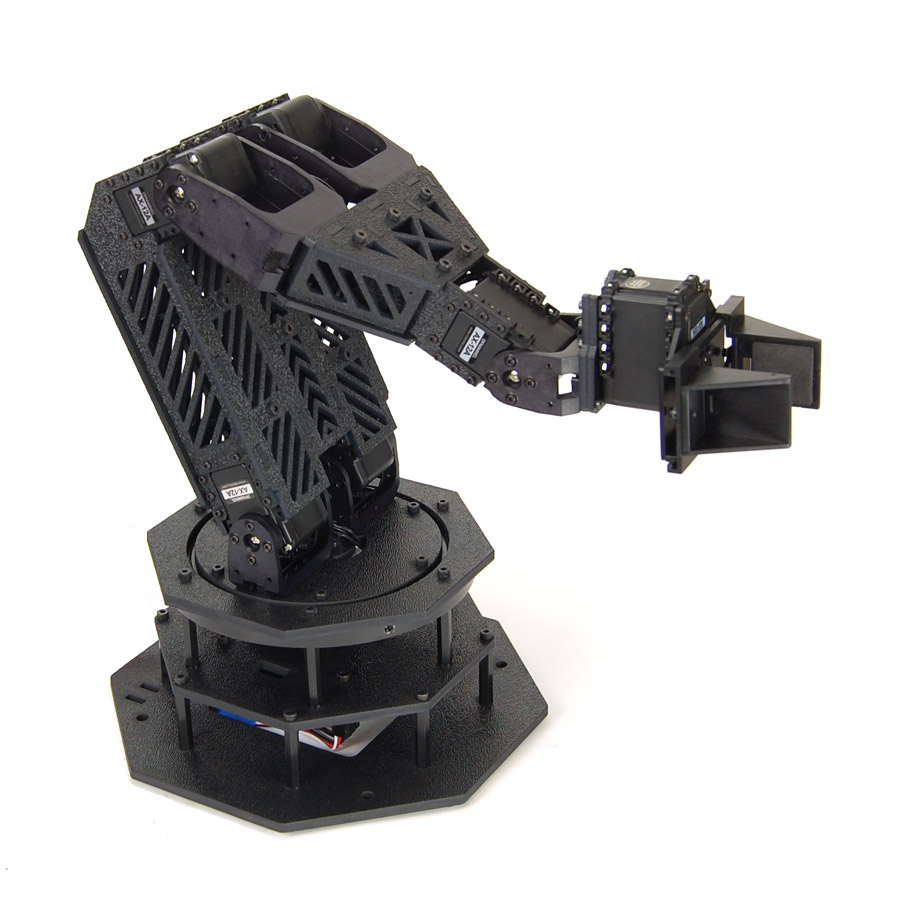
\includegraphics[scale=0.35]{arm}
\caption{Trossenrobotics Reactor.}
\end{figure}

\subsection{Hårdvara}

Till styrenheten krävs följande hårdvara.
\begin{itemize}
\item{2 hjulpar.}
\item{En AVR av typ Atmega16.}
\item{En Trossenrobotics Reactor.}
\end{itemize}

\subsection{Mjukvara}

Mjukvaran på Styrenheten kommer att vara främst avbrottsstyrd. Figur \ref{motor-interrupt-figure} illustrerar programflödet för avbrott. Vid kommando för att sätta register kommer ett servos målposition att uppdateras i ett separat register. Vid kommando för att utföra kommandon kommer servonas interna register för målposition att uppdateras med den information som fåtts av föregående avbrott. \\

\begin{figure}
\centering
\begin{minipage}[b]{.5\linewidth}
\centering
\scalebox{0.7}{% Graphic for TeX using PGF
% Title: /home/hannes/GitHub/TSEA29/dokumentation/designspecifikation/motor-flow-interrupt.dia
% Creator: Dia v0.97.2
% CreationDate: Tue Oct  7 23:01:32 2014
% For: hannes
% \usepackage{tikz}
% The following commands are not supported in PSTricks at present
% We define them conditionally, so when they are implemented,
% this pgf file will use them.
\ifx\du\undefined
  \newlength{\du}
\fi
\setlength{\du}{15\unitlength}
\begin{tikzpicture}
\pgftransformxscale{1.000000}
\pgftransformyscale{-1.000000}
\definecolor{dialinecolor}{rgb}{0.000000, 0.000000, 0.000000}
\pgfsetstrokecolor{dialinecolor}
\definecolor{dialinecolor}{rgb}{1.000000, 1.000000, 1.000000}
\pgfsetfillcolor{dialinecolor}
\definecolor{dialinecolor}{rgb}{1.000000, 1.000000, 1.000000}
\pgfsetfillcolor{dialinecolor}
\fill (17.531200\du,5.665170\du)--(17.531200\du,8.640170\du)--(28.181200\du,8.640170\du)--(28.181200\du,5.665170\du)--cycle;
\pgfsetlinewidth{0.100000\du}
\pgfsetdash{}{0pt}
\pgfsetdash{}{0pt}
\pgfsetmiterjoin
\definecolor{dialinecolor}{rgb}{0.000000, 0.000000, 0.000000}
\pgfsetstrokecolor{dialinecolor}
\draw (17.531200\du,5.665170\du)--(17.531200\du,8.640170\du)--(28.181200\du,8.640170\du)--(28.181200\du,5.665170\du)--cycle;
% setfont left to latex
\definecolor{dialinecolor}{rgb}{0.000000, 0.000000, 0.000000}
\pgfsetstrokecolor{dialinecolor}
\node at (22.856200\du,6.947670\du){Avbrott 1};
% setfont left to latex
\definecolor{dialinecolor}{rgb}{0.000000, 0.000000, 0.000000}
\pgfsetstrokecolor{dialinecolor}
\node at (22.856200\du,7.747670\du){Mottaget UART};
\definecolor{dialinecolor}{rgb}{1.000000, 1.000000, 1.000000}
\pgfsetfillcolor{dialinecolor}
\fill (17.593700\du,17.593735\du)--(17.593700\du,20.531235\du)--(28.118700\du,20.531235\du)--(28.118700\du,17.593735\du)--cycle;
\pgfsetlinewidth{0.100000\du}
\pgfsetdash{}{0pt}
\pgfsetdash{}{0pt}
\pgfsetmiterjoin
\definecolor{dialinecolor}{rgb}{0.000000, 0.000000, 0.000000}
\pgfsetstrokecolor{dialinecolor}
\draw (17.593700\du,17.593735\du)--(17.593700\du,20.531235\du)--(28.118700\du,20.531235\du)--(28.118700\du,17.593735\du)--cycle;
% setfont left to latex
\definecolor{dialinecolor}{rgb}{0.000000, 0.000000, 0.000000}
\pgfsetstrokecolor{dialinecolor}
\node at (22.856200\du,19.257485\du){Tolka kommando};
\definecolor{dialinecolor}{rgb}{1.000000, 1.000000, 1.000000}
\pgfsetfillcolor{dialinecolor}
\fill (17.631200\du,29.484800\du)--(17.631200\du,32.484800\du)--(28.081200\du,32.484800\du)--(28.081200\du,29.484800\du)--cycle;
\pgfsetlinewidth{0.100000\du}
\pgfsetdash{}{0pt}
\pgfsetdash{}{0pt}
\pgfsetmiterjoin
\definecolor{dialinecolor}{rgb}{0.000000, 0.000000, 0.000000}
\pgfsetstrokecolor{dialinecolor}
\draw (17.631200\du,29.484800\du)--(17.631200\du,32.484800\du)--(28.081200\du,32.484800\du)--(28.081200\du,29.484800\du)--cycle;
% setfont left to latex
\definecolor{dialinecolor}{rgb}{0.000000, 0.000000, 0.000000}
\pgfsetstrokecolor{dialinecolor}
\node at (22.856200\du,31.179800\du){Utför kommando};
\definecolor{dialinecolor}{rgb}{1.000000, 1.000000, 1.000000}
\pgfsetfillcolor{dialinecolor}
\fill (28.685600\du,11.639200\du)--(28.685600\du,14.589200\du)--(35.050000\du,14.589200\du)--(35.050000\du,11.639200\du)--cycle;
\pgfsetlinewidth{0.100000\du}
\pgfsetdash{}{0pt}
\pgfsetdash{}{0pt}
\pgfsetmiterjoin
\definecolor{dialinecolor}{rgb}{0.000000, 0.000000, 0.000000}
\pgfsetstrokecolor{dialinecolor}
\draw (28.685600\du,11.639200\du)--(28.685600\du,14.589200\du)--(35.050000\du,14.589200\du)--(35.050000\du,11.639200\du)--cycle;
% setfont left to latex
\definecolor{dialinecolor}{rgb}{0.000000, 0.000000, 0.000000}
\pgfsetstrokecolor{dialinecolor}
\node at (31.867800\du,13.309200\du){Lagra data};
\definecolor{dialinecolor}{rgb}{1.000000, 1.000000, 1.000000}
\pgfsetfillcolor{dialinecolor}
\fill (22.856200\du,21.555352\du)--(26.636530\du,25.008017\du)--(22.856200\du,28.460683\du)--(19.075870\du,25.008017\du)--cycle;
\pgfsetlinewidth{0.100000\du}
\pgfsetdash{}{0pt}
\pgfsetdash{}{0pt}
\pgfsetmiterjoin
\definecolor{dialinecolor}{rgb}{0.000000, 0.000000, 0.000000}
\pgfsetstrokecolor{dialinecolor}
\draw (22.856200\du,21.555352\du)--(26.636530\du,25.008017\du)--(22.856200\du,28.460683\du)--(19.075870\du,25.008017\du)--cycle;
% setfont left to latex
\definecolor{dialinecolor}{rgb}{0.000000, 0.000000, 0.000000}
\pgfsetstrokecolor{dialinecolor}
\node at (22.856200\du,25.203017\du){Väntas data?};
\definecolor{dialinecolor}{rgb}{1.000000, 1.000000, 1.000000}
\pgfsetfillcolor{dialinecolor}
\fill (28.717800\du,23.558000\du)--(28.717800\du,26.558000\du)--(35.017800\du,26.558000\du)--(35.017800\du,23.558000\du)--cycle;
\pgfsetlinewidth{0.100000\du}
\pgfsetdash{}{0pt}
\pgfsetdash{}{0pt}
\pgfsetmiterjoin
\definecolor{dialinecolor}{rgb}{0.000000, 0.000000, 0.000000}
\pgfsetstrokecolor{dialinecolor}
\draw (28.717800\du,23.558000\du)--(28.717800\du,26.558000\du)--(35.017800\du,26.558000\du)--(35.017800\du,23.558000\du)--cycle;
% setfont left to latex
\definecolor{dialinecolor}{rgb}{0.000000, 0.000000, 0.000000}
\pgfsetstrokecolor{dialinecolor}
\node at (31.867800\du,25.253000\du){Vänta på data};
\pgfsetlinewidth{0.100000\du}
\pgfsetdash{}{0pt}
\pgfsetdash{}{0pt}
\pgfsetbuttcap
{
\definecolor{dialinecolor}{rgb}{0.000000, 0.000000, 0.000000}
\pgfsetfillcolor{dialinecolor}
% was here!!!
\definecolor{dialinecolor}{rgb}{0.000000, 0.000000, 0.000000}
\pgfsetstrokecolor{dialinecolor}
\draw (22.856200\du,8.640170\du)--(22.856200\du,9.664287\du);
}
\pgfsetlinewidth{0.100000\du}
\pgfsetdash{}{0pt}
\pgfsetdash{}{0pt}
\pgfsetbuttcap
{
\definecolor{dialinecolor}{rgb}{0.000000, 0.000000, 0.000000}
\pgfsetfillcolor{dialinecolor}
% was here!!!
\definecolor{dialinecolor}{rgb}{0.000000, 0.000000, 0.000000}
\pgfsetstrokecolor{dialinecolor}
\draw (22.856200\du,16.569618\du)--(22.856200\du,17.593735\du);
}
\pgfsetlinewidth{0.100000\du}
\pgfsetdash{}{0pt}
\pgfsetdash{}{0pt}
\pgfsetbuttcap
{
\definecolor{dialinecolor}{rgb}{0.000000, 0.000000, 0.000000}
\pgfsetfillcolor{dialinecolor}
% was here!!!
\definecolor{dialinecolor}{rgb}{0.000000, 0.000000, 0.000000}
\pgfsetstrokecolor{dialinecolor}
\draw (22.856200\du,20.531235\du)--(22.856200\du,21.555352\du);
}
\pgfsetlinewidth{0.100000\du}
\pgfsetdash{}{0pt}
\pgfsetdash{}{0pt}
\pgfsetbuttcap
{
\definecolor{dialinecolor}{rgb}{0.000000, 0.000000, 0.000000}
\pgfsetfillcolor{dialinecolor}
% was here!!!
\definecolor{dialinecolor}{rgb}{0.000000, 0.000000, 0.000000}
\pgfsetstrokecolor{dialinecolor}
\draw (22.856200\du,28.460683\du)--(22.856200\du,29.484800\du);
}
\pgfsetlinewidth{0.100000\du}
\pgfsetdash{}{0pt}
\pgfsetdash{}{0pt}
\pgfsetbuttcap
{
\definecolor{dialinecolor}{rgb}{0.000000, 0.000000, 0.000000}
\pgfsetfillcolor{dialinecolor}
% was here!!!
\definecolor{dialinecolor}{rgb}{0.000000, 0.000000, 0.000000}
\pgfsetstrokecolor{dialinecolor}
\draw (26.636530\du,13.116952\du)--(28.685600\du,13.114200\du);
}
\pgfsetlinewidth{0.100000\du}
\pgfsetdash{}{0pt}
\pgfsetdash{}{0pt}
\pgfsetbuttcap
{
\definecolor{dialinecolor}{rgb}{0.000000, 0.000000, 0.000000}
\pgfsetfillcolor{dialinecolor}
% was here!!!
\definecolor{dialinecolor}{rgb}{0.000000, 0.000000, 0.000000}
\pgfsetstrokecolor{dialinecolor}
\draw (26.636530\du,25.008017\du)--(28.717800\du,25.058000\du);
}
\definecolor{dialinecolor}{rgb}{1.000000, 1.000000, 1.000000}
\pgfsetfillcolor{dialinecolor}
\fill (22.856200\du,9.664287\du)--(26.636530\du,13.116952\du)--(22.856200\du,16.569618\du)--(19.075870\du,13.116952\du)--cycle;
\pgfsetlinewidth{0.100000\du}
\pgfsetdash{}{0pt}
\pgfsetdash{}{0pt}
\pgfsetmiterjoin
\definecolor{dialinecolor}{rgb}{0.000000, 0.000000, 0.000000}
\pgfsetstrokecolor{dialinecolor}
\draw (22.856200\du,9.664287\du)--(26.636530\du,13.116952\du)--(22.856200\du,16.569618\du)--(19.075870\du,13.116952\du)--cycle;
% setfont left to latex
\definecolor{dialinecolor}{rgb}{0.000000, 0.000000, 0.000000}
\pgfsetstrokecolor{dialinecolor}
\node at (22.856200\du,12.911952\du){Mottaget};
% setfont left to latex
\definecolor{dialinecolor}{rgb}{0.000000, 0.000000, 0.000000}
\pgfsetstrokecolor{dialinecolor}
\node at (22.856200\du,13.711952\du){Kommando?};
% setfont left to latex
\definecolor{dialinecolor}{rgb}{0.000000, 0.000000, 0.000000}
\pgfsetstrokecolor{dialinecolor}
\node[anchor=west] at (26.700000\du,11.950000\du){Ja};
% setfont left to latex
\definecolor{dialinecolor}{rgb}{0.000000, 0.000000, 0.000000}
\pgfsetstrokecolor{dialinecolor}
\node[anchor=west] at (23.400000\du,17.050000\du){Nej};
% setfont left to latex
\definecolor{dialinecolor}{rgb}{0.000000, 0.000000, 0.000000}
\pgfsetstrokecolor{dialinecolor}
\node[anchor=west] at (26.850000\du,24.350000\du){Ja};
% setfont left to latex
\definecolor{dialinecolor}{rgb}{0.000000, 0.000000, 0.000000}
\pgfsetstrokecolor{dialinecolor}
\node[anchor=west] at (23.250000\du,29.050000\du){Nej};
\end{tikzpicture}
}
\subcaption{Flödesschema för avbrottsrutin}\label{designspec:motor-interrupt-figure}
\end{minipage}%
\begin{minipage}[b]{.5\linewidth}
\centering
\scalebox{0.7}{% Graphic for TeX using PGF
% Title: /home/hannes/GitHub/TSEA29/dokumentation/designspecifikation/motor-flow-main.dia
% Creator: Dia v0.97.2
% CreationDate: Tue Oct  7 16:02:05 2014
% For: hannes
% \usepackage{tikz}
% The following commands are not supported in PSTricks at present
% We define them conditionally, so when they are implemented,
% this pgf file will use them.
\ifx\du\undefined
  \newlength{\du}
\fi
\setlength{\du}{15\unitlength}
\begin{tikzpicture}
\pgftransformxscale{1.000000}
\pgftransformyscale{-1.000000}
\definecolor{dialinecolor}{rgb}{0.000000, 0.000000, 0.000000}
\pgfsetstrokecolor{dialinecolor}
\definecolor{dialinecolor}{rgb}{1.000000, 1.000000, 1.000000}
\pgfsetfillcolor{dialinecolor}
\definecolor{dialinecolor}{rgb}{1.000000, 1.000000, 1.000000}
\pgfsetfillcolor{dialinecolor}
\fill (21.347417\du,3.644670\du)--(24.727748\du,6.097335\du)--(21.347417\du,8.550000\du)--(17.967087\du,6.097335\du)--cycle;
\pgfsetlinewidth{0.100000\du}
\pgfsetdash{}{0pt}
\pgfsetdash{}{0pt}
\pgfsetmiterjoin
\definecolor{dialinecolor}{rgb}{0.000000, 0.000000, 0.000000}
\pgfsetstrokecolor{dialinecolor}
\draw (21.347417\du,3.644670\du)--(24.727748\du,6.097335\du)--(21.347417\du,8.550000\du)--(17.967087\du,6.097335\du)--cycle;
% setfont left to latex
\definecolor{dialinecolor}{rgb}{0.000000, 0.000000, 0.000000}
\pgfsetstrokecolor{dialinecolor}
\node at (21.347417\du,6.292335\du){Start};
\definecolor{dialinecolor}{rgb}{1.000000, 1.000000, 1.000000}
\pgfsetfillcolor{dialinecolor}
\fill (17.797417\du,10.731000\du)--(17.797417\du,13.431000\du)--(24.897417\du,13.431000\du)--(24.897417\du,10.731000\du)--cycle;
\pgfsetlinewidth{0.100000\du}
\pgfsetdash{}{0pt}
\pgfsetdash{}{0pt}
\pgfsetmiterjoin
\definecolor{dialinecolor}{rgb}{0.000000, 0.000000, 0.000000}
\pgfsetstrokecolor{dialinecolor}
\draw (17.797417\du,10.731000\du)--(17.797417\du,13.431000\du)--(24.897417\du,13.431000\du)--(24.897417\du,10.731000\du)--cycle;
% setfont left to latex
\definecolor{dialinecolor}{rgb}{0.000000, 0.000000, 0.000000}
\pgfsetstrokecolor{dialinecolor}
\node at (21.347417\du,12.276000\du){Initiera};
\definecolor{dialinecolor}{rgb}{1.000000, 1.000000, 1.000000}
\pgfsetfillcolor{dialinecolor}
\fill (17.797417\du,14.549500\du)--(17.797417\du,17.249500\du)--(24.897417\du,17.249500\du)--(24.897417\du,14.549500\du)--cycle;
\pgfsetlinewidth{0.100000\du}
\pgfsetdash{}{0pt}
\pgfsetdash{}{0pt}
\pgfsetmiterjoin
\definecolor{dialinecolor}{rgb}{0.000000, 0.000000, 0.000000}
\pgfsetstrokecolor{dialinecolor}
\draw (17.797417\du,14.549500\du)--(17.797417\du,17.249500\du)--(24.897417\du,17.249500\du)--(24.897417\du,14.549500\du)--cycle;
% setfont left to latex
\definecolor{dialinecolor}{rgb}{0.000000, 0.000000, 0.000000}
\pgfsetstrokecolor{dialinecolor}
\node at (21.347417\du,15.694500\du){Hämta status för };
% setfont left to latex
\definecolor{dialinecolor}{rgb}{0.000000, 0.000000, 0.000000}
\pgfsetstrokecolor{dialinecolor}
\node at (21.347417\du,16.494500\du){servon};
\definecolor{dialinecolor}{rgb}{1.000000, 1.000000, 1.000000}
\pgfsetfillcolor{dialinecolor}
\fill (17.797417\du,22.186500\du)--(17.797417\du,24.886500\du)--(24.897417\du,24.886500\du)--(24.897417\du,22.186500\du)--cycle;
\pgfsetlinewidth{0.100000\du}
\pgfsetdash{}{0pt}
\pgfsetdash{}{0pt}
\pgfsetmiterjoin
\definecolor{dialinecolor}{rgb}{0.000000, 0.000000, 0.000000}
\pgfsetstrokecolor{dialinecolor}
\draw (17.797417\du,22.186500\du)--(17.797417\du,24.886500\du)--(24.897417\du,24.886500\du)--(24.897417\du,22.186500\du)--cycle;
% setfont left to latex
\definecolor{dialinecolor}{rgb}{0.000000, 0.000000, 0.000000}
\pgfsetstrokecolor{dialinecolor}
\node at (21.347417\du,23.331500\du){Beräkna nästa};
% setfont left to latex
\definecolor{dialinecolor}{rgb}{0.000000, 0.000000, 0.000000}
\pgfsetstrokecolor{dialinecolor}
\node at (21.347417\du,24.131500\du){hastigheter};
\definecolor{dialinecolor}{rgb}{1.000000, 1.000000, 1.000000}
\pgfsetfillcolor{dialinecolor}
\fill (17.797417\du,26.005000\du)--(17.797417\du,28.705000\du)--(24.897417\du,28.705000\du)--(24.897417\du,26.005000\du)--cycle;
\pgfsetlinewidth{0.100000\du}
\pgfsetdash{}{0pt}
\pgfsetdash{}{0pt}
\pgfsetmiterjoin
\definecolor{dialinecolor}{rgb}{0.000000, 0.000000, 0.000000}
\pgfsetstrokecolor{dialinecolor}
\draw (17.797417\du,26.005000\du)--(17.797417\du,28.705000\du)--(24.897417\du,28.705000\du)--(24.897417\du,26.005000\du)--cycle;
% setfont left to latex
\definecolor{dialinecolor}{rgb}{0.000000, 0.000000, 0.000000}
\pgfsetstrokecolor{dialinecolor}
\node at (21.347417\du,27.150000\du){Uppdatera};
% setfont left to latex
\definecolor{dialinecolor}{rgb}{0.000000, 0.000000, 0.000000}
\pgfsetstrokecolor{dialinecolor}
\node at (21.347417\du,27.950000\du){hastigheter};
\pgfsetlinewidth{0.100000\du}
\pgfsetdash{}{0pt}
\pgfsetdash{}{0pt}
\pgfsetbuttcap
{
\definecolor{dialinecolor}{rgb}{0.000000, 0.000000, 0.000000}
\pgfsetfillcolor{dialinecolor}
% was here!!!
\definecolor{dialinecolor}{rgb}{0.000000, 0.000000, 0.000000}
\pgfsetstrokecolor{dialinecolor}
\draw (21.347417\du,8.550000\du)--(21.347417\du,10.731000\du);
}
\pgfsetlinewidth{0.100000\du}
\pgfsetdash{}{0pt}
\pgfsetdash{}{0pt}
\pgfsetbuttcap
{
\definecolor{dialinecolor}{rgb}{0.000000, 0.000000, 0.000000}
\pgfsetfillcolor{dialinecolor}
% was here!!!
\definecolor{dialinecolor}{rgb}{0.000000, 0.000000, 0.000000}
\pgfsetstrokecolor{dialinecolor}
\draw (21.347417\du,13.431000\du)--(21.347417\du,14.549500\du);
}
\pgfsetlinewidth{0.100000\du}
\pgfsetdash{}{0pt}
\pgfsetdash{}{0pt}
\pgfsetbuttcap
{
\definecolor{dialinecolor}{rgb}{0.000000, 0.000000, 0.000000}
\pgfsetfillcolor{dialinecolor}
% was here!!!
\definecolor{dialinecolor}{rgb}{0.000000, 0.000000, 0.000000}
\pgfsetstrokecolor{dialinecolor}
\draw (21.347417\du,24.886500\du)--(21.347417\du,26.005000\du);
}
\pgfsetlinewidth{0.100000\du}
\pgfsetdash{}{0pt}
\pgfsetdash{}{0pt}
\pgfsetmiterjoin
\pgfsetbuttcap
{
\definecolor{dialinecolor}{rgb}{0.000000, 0.000000, 0.000000}
\pgfsetfillcolor{dialinecolor}
% was here!!!
{\pgfsetcornersarced{\pgfpoint{0.000000\du}{0.000000\du}}\definecolor{dialinecolor}{rgb}{0.000000, 0.000000, 0.000000}
\pgfsetstrokecolor{dialinecolor}
\draw (21.347417\du,28.705000\du)--(21.400000\du,30.000000\du)--(14.400000\du,30.000000\du)--(14.450000\du,14.050000\du)--(21.347417\du,13.990250\du);
}}
\definecolor{dialinecolor}{rgb}{1.000000, 1.000000, 1.000000}
\pgfsetfillcolor{dialinecolor}
\fill (17.797417\du,18.368000\du)--(17.797417\du,21.068000\du)--(24.897417\du,21.068000\du)--(24.897417\du,18.368000\du)--cycle;
\pgfsetlinewidth{0.100000\du}
\pgfsetdash{}{0pt}
\pgfsetdash{}{0pt}
\pgfsetmiterjoin
\definecolor{dialinecolor}{rgb}{0.000000, 0.000000, 0.000000}
\pgfsetstrokecolor{dialinecolor}
\draw (17.797417\du,18.368000\du)--(17.797417\du,21.068000\du)--(24.897417\du,21.068000\du)--(24.897417\du,18.368000\du)--cycle;
% setfont left to latex
\definecolor{dialinecolor}{rgb}{0.000000, 0.000000, 0.000000}
\pgfsetstrokecolor{dialinecolor}
\node at (21.347417\du,19.513000\du){Om arm-rörelse};
% setfont left to latex
\definecolor{dialinecolor}{rgb}{0.000000, 0.000000, 0.000000}
\pgfsetstrokecolor{dialinecolor}
\node at (21.347417\du,20.313000\du){klar, sätt busy=1};
\pgfsetlinewidth{0.100000\du}
\pgfsetdash{}{0pt}
\pgfsetdash{}{0pt}
\pgfsetbuttcap
{
\definecolor{dialinecolor}{rgb}{0.000000, 0.000000, 0.000000}
\pgfsetfillcolor{dialinecolor}
% was here!!!
\definecolor{dialinecolor}{rgb}{0.000000, 0.000000, 0.000000}
\pgfsetstrokecolor{dialinecolor}
\draw (21.347417\du,17.249500\du)--(21.347417\du,18.368000\du);
}
\pgfsetlinewidth{0.100000\du}
\pgfsetdash{}{0pt}
\pgfsetdash{}{0pt}
\pgfsetbuttcap
{
\definecolor{dialinecolor}{rgb}{0.000000, 0.000000, 0.000000}
\pgfsetfillcolor{dialinecolor}
% was here!!!
\definecolor{dialinecolor}{rgb}{0.000000, 0.000000, 0.000000}
\pgfsetstrokecolor{dialinecolor}
\draw (21.347417\du,21.068000\du)--(21.347417\du,22.186500\du);
}
\end{tikzpicture}
}
\subcaption{Flödesschema för mainloop}\label{designspec:motor-main-figure}
\end{minipage}
\caption{Styrenhetens mjukvara}\label{fig:1}
\end{figure}

När AVRen inte är upptagen med avbrott körs en loop där alla servons hastighet och position läses av, jämförs med dess målposition och uppdateras med en ny hastighet. Figur \ref{motor-main-figure} illustrerar programflödet. Detta ger oss den smoothing-effekt vi söker. \\
Vid de tillfällen AVRen kommunicerar med servon genom UART bör alla avbrott slås av.  \\

\newpage
\begin{appendices}

% Bilagor

\end{appendices}


\end{document}
